\documentclass[12pt]{report}

% Packages
\usepackage[a4paper, top=1in, bottom=1in, left=1.5in, right=1in]{geometry}  % 1-inch margins
\usepackage{setspace}  % Line spacing
\usepackage{graphicx}
\usepackage{titlesec} 
\usepackage{acronym}
\usepackage{changepage}
\usepackage{indentfirst}
\usepackage{float}
\usepackage{multirow}
\usepackage{booktabs}
\usepackage{amsmath}
\usepackage{amsfonts}
\usepackage{tikz}
\usepackage{newtxtext,newtxmath}




\usepackage[style=apa, backend=biber]{biblatex}
\addbibresource{ref.bib}



\setcounter{secnumdepth}{4}
\linespread{1.5}


% Center Chapter Titles
\titleformat{\chapter}[display]
  {\normalfont\LARGE\bfseries\centering} % Large bold centered title
  {\chaptername\ \thechapter}{20pt}{\LARGE}

% Title Page



\begin{document}

\begin{titlepage}
    \centering

    
    {\fontsize{16pt}{19pt}\selectfont \textbf{Enhancing Sleep Stage Classification with}}\\
    {\fontsize{16pt}{19pt}\selectfont \textbf{Vision Transformers}} \\ [0.4 cm]
    {\fontsize{16pt}{19pt}\selectfont \textbf{A Study on Image Transformations, Data Augmentation, and Model Optimization}}\\

    \vfill

    
    {\fontsize{12pt}{15pt}\selectfont By}\\
    {\fontsize{14pt}{17pt}\selectfont \textbf{H.R.J.R. Rashmika}}\\

    \vfill
    
    \fontsize{12pt}{14pt}\selectfont This dissertation is submitted as a partial fulfillment of the\\
    {\fontsize{12pt}{14pt}\selectfont \textbf{B.Sc. (Hons) in Data Science}}\\ [1 cm]

    
    {\fontsize{14pt}{17pt}\selectfont Department of Statistics}\\
    {\fontsize{14pt}{17pt}\selectfont University of Colombo, Sri Lanka}\\ [1 cm]

    
    {\fontsize{12pt}{14pt}\selectfont March 2025}\\

\end{titlepage}





\pagenumbering{roman}

%\maketitle

\chapter*{Abstract}
\addcontentsline{toc}{section}{Abstract}

{\setlength{\parindent}{0pt}
Sleep stage classification is essential for diagnosing sleep disorders and analyzing sleep patterns. This study investigates the effectiveness of Vision Transformers (ViTs) for sleep stage classification using EEG-based image transformations. Multiple transformation techniques, including Spectrograms, Gramian Angular Fields (GADF, GASF), and Markov Transition Fields (MTF), are evaluated to identify the most suitable representation. Additionally, the impact of different sampling frequencies and resampling methods is examined. \\

To mitigate class imbalance and subject variability, a Deep Convolutional Generative Adversarial Network (DCGAN) is employed to generate synthetic sleep stage images. The effectiveness of GAN-augmented data is assessed by comparing classification performance on datasets with and without synthetic samples. Furthermore, we compare ViTs trained from scratch versus pre-trained ViTs and evaluate various pre-trained models to determine the optimal architecture. \\

Experimental results show that GASF with Discrete Wavelet Transform (DWT) at 128 Hz yields the best classification performance. GAN-based augmentation improves accuracy by enhancing dataset diversity. The final model, ViT-B/16 fine-tuned on augmented data, achieves the highest classification accuracy  84.8\% and generalizes well across independent datasets. These findings highlight the potential of Vision Transformers in advancing automated sleep stage classification. \\

\textbf{Keywords:} Sleep stage classification, Vision Transformers, EEG, Image transformation, GAN, Deep learning, Data augmentation.
}

\chapter*{Declaration}
\addcontentsline{toc}{section}{Declaration}

{\setlength{\parindent}{0pt}
This thesis is my original work and has not been submitted previously for a degree at this or any other university/institute. To the best of my knowledge, it does not contain any material published or written by another person, except as acknowledged in the text.\\ [0.5 cm]

\noindent
\textbf{Candidate:}    \hspace{3.75cm} \textbf{Signature:} \underline{\hspace{6cm}}  \\
H.R.J.R. Rashmika
\vspace{0.5cm}

\noindent
\hspace{6cm}  \textbf{Date:} \underline{\hspace{7cm}} 

\vspace{1cm}

This is to certify that this dissertation is based on the work carried out by Mr. H.R.J.R. Rashmika under my supervision. This dissertation has been prepared according to the format stipulated and is of acceptable standard.\\ [0.5 cm]

\noindent
\textbf{Supervisor:}    \hspace{3.56cm} \textbf{Signature:} \underline{\hspace{6cm}}  
\hspace{8.25cm} Dr. G.A.C.N. Priyadarshani, \\
\hspace{8.25cm} Senior lecturer, \\
\hspace{8.25cm} Department of Statistics,  \\
\hspace{8.25cm} University of Colombo. \hspace{2.3cm} \textbf{Date:} \underline{\hspace{7cm}} \\

}


\tableofcontents
\addcontentsline{toc}{section}{Table of contents}

\listoffigures 
\addcontentsline{toc}{section}{List of Figures}

\listoftables   
\addcontentsline{toc}{section}{List of Tables}

\chapter*{Acronyms}
\begin{acronym}


\acro{AASM}{American Academy of Sleep Medicine}

\acro{cGAN}{Conditional GAN}
\acro{CHI}{Calinski-Harabasz Index}
\acro{CNN}{Convolutional Neural Network}
\acro{CWT}{Continuous Wavelet Transform}

\acro{DBI}{Davies-Bouldin Index}
\acro{DCGAN}{Deep Convolutional GAN}

\acro{ECG}{Electrocardiography}
\acro{EEG}{Electroencephalography}
\acro{EKG}{Electrocardiogram}
\acro{EMG}{Electromyography}
\acro{EOG}{Electrooculography}

\acro{FID}{Fr´echet Inception Distance}

\acro{GAF}{Gramian Angular Fields}
\acro{GAN}{Generative Adversarial Network}

\acro{HHT}{Hilbert-Huang Transform}
\acro{HMM}{Hidden Markov Model}

\acro{KNN}{k-Nearest Neighbors}

\acro{LRP}{Layer-wise Relevance Propagation}
\acro{LSTM}{Long-Short Term Memory}

\acro{MPED}{Mean Pairwise Euclidean Distance}
\acro{MTF}{Markov Transition Fields}


\acro{NLP}{Natural Language Processing}
\acro{NREM}{Non Rapid Eye Movement }

\acro{PSD}{Power Spectral Density}
\acro{PSG}{Polysomnography}

\acro{REM}{Rapid Eye Movement}
\acro{RNN}{Recurrent Neural Network}

\acro{SSIM}{Structural Similarity Index}
\acro{STFT}{Short Time Fourier Transform}
\acro{SVM}{Support Vector Machine}

\acro{t-SNE}{t-Distributed Stochastic Neighbor}

\acro{ViT}{Vision Transformer}


\end{acronym}


\pagenumbering{arabic}

\chapter{Introduction}

%--------------------------------------------------------------------------------------------------------
\section{Motivation}

Humans spend nearly one-third of their lives sleeping, highlighting its essential role in maintaining physical and cognitive well-being. Sleep is fundamental for brain development, memory consolidation, emotional regulation, and immune system function. However, disruptions in sleep quality and duration have been linked to various health issues, including cardiovascular diseases, obesity, diabetes, neurodegenerative disorders, and mental health conditions such as anxiety and depression \parencite{itani2017short}.\\

Despite its importance, sleep disorders are becoming increasingly prevalent, with conditions such as insomnia, sleep apnea, and narcolepsy affecting millions of individuals worldwide. It is estimated that around 50–70 million adults in the United States alone suffer from chronic sleep disorders, while an even larger population experiences occasional sleep disturbances. The growing burden of these disorders presents a significant public health concern, as inadequate sleep is associated with reduced productivity, impaired cognitive function, and increased healthcare costs \parencite{hirshkowitz2015national}.\\

Accurate sleep stage classification is a crucial step in diagnosing sleep disorders and understanding individual sleep patterns. Traditionally, sleep stage scoring relies on \ac{PSG} data, which requires trained specialists to manually annotate sleep stages based on recorded physiological signals. This manual process is labor-intensive, time-consuming, and subject to variability between scorers \parencite{yildirim2019deep}. To address these limitations, researchers have been actively exploring automated methods for sleep stage classification using machine learning and deep learning techniques \parencite{ardeshir2023sleep}.\\

To address the growing global burden of sleep disorders and the limitations of current diagnostic methods, there is a critical need for reliable, automated solutions that can support large-scale and long-term sleep monitoring. The motivation behind this study lies in the pursuit of more accessible, accurate, and scalable tools for sleep stage classification tools that can reduce the reliance on manual scoring and extend diagnostic capabilities beyond clinical settings. By leveraging recent advances in deep learning, particularly architectures capable of capturing intricate patterns in physiological data, this research aims to push the boundaries of automated sleep analysis. In doing so, it seeks to contribute meaningfully to early detection, personalized treatment, and improved outcomes for individuals affected by sleep-related conditions.
%--------------------------------------------------------------------------------------------------------
\section{Background}

\subsection{Foundations of Sleep Monitoring}

Understanding sleep and its underlying mechanisms requires a multidisciplinary perspective, drawing from neuroscience, electrophysiology, and biomedical engineering. The process of monitoring sleep is deeply rooted in our understanding of brain anatomy, how neural signals are generated and transmitted, and how they can be recorded and interpreted using various physiological monitoring techniques. \\

The brain is the central organ of the human nervous system, responsible for regulating thought, emotion, sensory perception, and motor functions. Alongside the spinal cord, it forms the central nervous system (CNS), managing both voluntary and involuntary processes essential for survival and homeostasis. \\

As illustrated in Figure \ref{fig:brain_structure}, the brain consists of three major regions: the cerebrum, cerebellum, and brainstem, each playing a vital role in maintaining physiological stability \parencite{kandel2000principles}. The cerebrum, the largest part, handles higher-order functions such as reasoning, memory, sensory processing, and voluntary movement. Beneath it, the cerebellum fine-tunes motor activity and supports balance and coordination. The brainstem, connecting the brain to the spinal cord, controls autonomic functions like breathing and heart rate \parencite{purves2013principles}.

\begin{figure}[H]
    \centering
    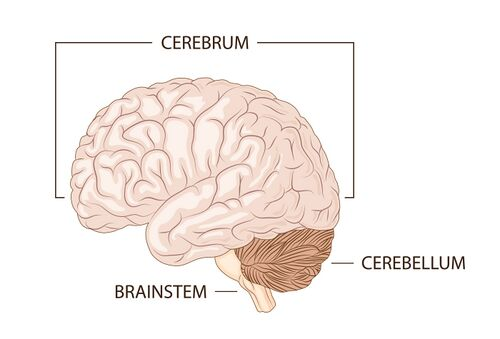
\includegraphics[width=0.55\linewidth]{Figures/Brain_anatomy.jpeg}
    \caption{Structural Organization of the Human Brain}
    \label{fig:brain_structure}
\end{figure}

The cerebral cortex, the brain’s outer layer, is shown in Figure \ref{fig:brain_2h_4l} and is divided into the left and right hemispheres. Each hemisphere contains four lobes frontal, parietal, temporal, and occipital each associated with specific cognitive and sensory roles. These anatomical divisions are especially relevant in sleep studies, as they contribute to distinct neural activities during different sleep stages.

\begin{figure}[H]
    \centering
    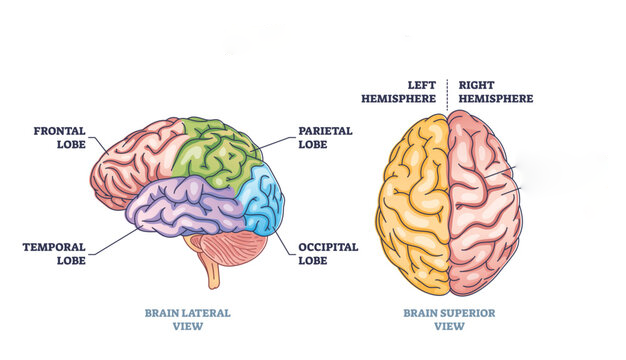
\includegraphics[width=0.6\linewidth]{Figures/brain 2h 4l.png}
    \caption{Structural division of the Brain into Lobes and Hemispheres}
    \label{fig:brain_2h_4l}
\end{figure}

Building upon the structural and functional overview of the brain, understanding how it generates and transmits signals is essential for interpreting the neural activity associated with sleep. Brain function relies on the communication between neurons specialized cells that transmit information via electrical and chemical signals. Neurons transmit information through action potentials, brief electrical impulses triggered by ion movement across the cell membrane. These signals travel along axons and activate neurotransmitter release at synapses, enabling communication across brain regions \parencite{bear2020neuroscience}. \\

To observe this activity, various techniques measure brain signals at different spatial and temporal resolutions. Among them, Electroencephalography (EEG) is particularly effective in sleep research, offering real-time insights into the brain’s electrical activity. EEG measures electrical activity from cortical neurons using electrodes placed on the scalp. These electrodes detect potential differences resulting from synchronized post-synaptic activity. As the raw signals are subtle, they are amplified and digitized for meaningful analysis \parencite{niedermeyer2005electroencephalography}. \\

\begin{figure}[H]
    \centering
    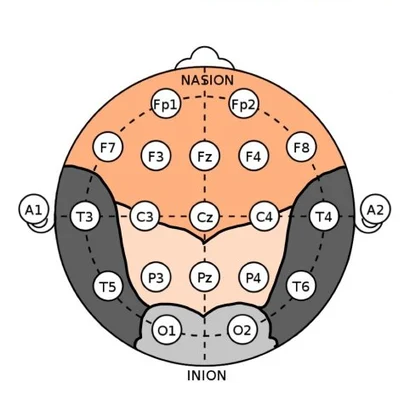
\includegraphics[width=0.65\linewidth]{Figures/the-10-20-system.png}
    \caption{The international 10-20 system for electrodes placement}
    \label{fig:the-10-20-system}
\end{figure}

To standardize data collection, EEG setups typically follow the 10–20 International System (Figure \ref{fig:the-10-20-system}), which positions electrodes based on skull landmarks. Electrodes are labeled by region F (frontal), C (central), P (parietal), O (occipital) with odd numbers for the left hemisphere, even for the right, and 'z' for midline placements. \\

While EEG provides focused insights into brain activity, comprehensive sleep analysis requires monitoring multiple physiological systems. Polysomnography (PSG) addresses this need by integrating various biophysical measurements, making it the gold standard for assessing sleep architecture and diagnosing sleep disorders. A standard PSG setup includes:
\begin{enumerate}
    \item \aclabelfont{EEG} (\acl{EEG}): Measures electrical activity in the brain.
    \item \aclabelfont{EOG} (\acl{EOG}): Detects eye movements.
    \item \aclabelfont{EMG} (\acl{EMG}): Monitors muscle activity.
    \item \aclabelfont{ECG} (\acl{ECG}): Tracks the electrical activity of the heart.
    \item \textbf{Respiratory Monitoring}: Includes sensors to monitor airflow, chest movements, and blood oxygen levels, offering insights into breathing patterns and respiratory health.
    \item \textbf{Other Parameters}: Depending on the specific application, \ac{PSG} may also include monitoring of additional factors such as temperature, blood pressure, or body movements.
\end{enumerate}

As illustrated in Figure \ref{fig:psg_electrodes}, PSG captures a synchronized view of brain and body function during sleep. This rich dataset enables accurate staging and the identification of abnormalities.
 
\begin{figure}[H]
    \centering
    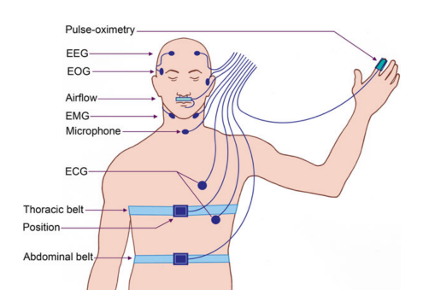
\includegraphics[width=0.65\linewidth]{Figures/psg.png}
    \caption{Electrode Placements for PSG Monitoring Across the Body}
    \label{fig:psg_electrodes}
\end{figure}
 
\subsection{Human Sleep}

Sleep is a fundamental biological process essential for maintaining overall health and cognitive function. It is a highly regulated state characterized by altered consciousness, reduced sensory perception, and diminished motor activity, allowing the body and brain to recover and process information. Contrary to being a passive state, sleep is an active and dynamic process involving complex physiological and neurological mechanisms. It plays a crucial role in cellular repair, immune system regulation, and metabolic homeostasis \parencite{walker2017we}.\\

Sleep is broadly classified into two main types: \ac{NREM} sleep and \ac{REM} sleep. These stages alternate cyclically throughout the night, forming sleep cycles that typically last between 90 and 120 minutes. A full night’s sleep consists of approximately four to six cycles, with the proportion of REM sleep increasing in later cycles, suggesting its critical role in cognitive processing and memory consolidation \parencite{carskadon2005normal}.\\

\ac{NREM} sleep accounts for approximately 75\%–80\% of total sleep and consists of three distinct stages. Stage 1 is a transitional phase between wakefulness and sleep, characterized by reduced muscle tone and slow eye movements. Stage 2 is marked by a decrease in body temperature and heart rate, with Sleep spindles and K-complexes observed in \ac{EEG} recordings, indicating the brain’s role in processing external stimuli and memory formation \parencite{de2003sleep}. Stage 3, also referred to as Deep sleep or Slow Wave Sleep, is the most restorative phase, playing a critical role in physical recovery, immune function, and long term memory consolidation \parencite{diekelmann2010memory}.\\

In contrast, REM sleep constitutes 20\%–25\% of total sleep and is characterized by rapid eye movements, vivid dreams, and heightened brain activity resembling wakefulness. This stage is essential for emotional regulation and cognitive functions such as problem-solving and creativity \parencite{bjorn2013sleep}. The dynamic alternation between NREM and REM sleep throughout the night reflects the brain's ongoing processes of neural reorganization and memory integration.\\

Brain wave activity during sleep varies across different stages, providing a reliable basis for identifying and classifying sleep phases. In the lighter stages of sleep, higher-frequency alpha and theta wavesdominate, signaling the brain’s gradual disengagement from external stimuli. These wave patterns are key indicators of early \ac{NREM} sleep. As sleep deepens, slow-wave delta activity becomes prominent, distinguishing Stage 3 sleep, which is essential for memory consolidation and tissue repair \parencite{sterpenich2007sleep}. During \ac{REM} sleep, a mixture of theta and beta waves emerges, resembling wakefulness and reflecting the brain's heightened activity associated with dreaming and cognitive processing \parencite{hobson2009rem}. By analyzing these characteristic neural oscillations, researchers can effectively classify sleep stages, aiding in the development of automated sleep staging models for clinical and research applications. Table \ref{tab:eeg_sleep_waves} presents the frequency bands of the characteristic wave types that occur during sleep.\\

\begin{table}[H]
    \centering
    \begin{tabular}{|c|c|}
        \hline
        \textbf{Wave Type} & \textbf{Frequency Range} \\ 
        \hline
        Slow-wave activity & 0.5–2 Hz \\ 
        \hline
        Delta waves & 0–3.99 Hz \\ 
        \hline
        Theta waves & 4–7.99 Hz \\ 
        \hline
        Alpha waves & 8–13 Hz \\ 
        \hline
        Beta waves & \textgreater 13 Hz \\ 
        \hline
    \end{tabular}
    \caption{EEG Frequency Bands Observed During Sleep}
    \label{tab:eeg_sleep_waves}
\end{table}

\subsection{Sleep Stages}

Human sleep, as discussed earlier, is a dynamic process consisting of distinct stages that cycle throughout the night. To systematically classify these stages, two widely recognized methodologies have been developed: the Rechtschaffen and Kales (R\&K) manual and the \ac{AASM} guidelines. While both methods aim to categorize sleep stages based on electrophysiological patterns, the R\&K system remains the most comprehensive and widely referenced framework due to its detailed classification and historical significance in sleep research \parencite{rechtschaffen1978techniques,iber2007aasm}.\\

The R\&K classification system, established in 1968, defines sleep architecture using \acs{EEG} (Electroencephalography), \acs{EOG} (Electrooculography), and \acs{EMG} (Electromyography) recordings. It divides sleep into five distinct stages:

\begin{enumerate}
    \item \textbf{NREM Stage 1}: This is the transition from wakefulness to sleep, lasting only a few minutes. It is characterized by low-amplitude, mixed-frequency brain waves (alpha and theta waves) \parencite{rechtschaffen1978techniques}. Slow rolling eye movements occur, and muscle activity decreases. The body begins to disengage from its surroundings in preparation for deeper sleep.

    \item \textbf{NREM Stage 2}: This stage makes up a significant portion of total sleep and is important for memory consolidation and sensory processing. It is marked by sleep spindles and K-complexes in \acs{EEG} recordings \parencite{de2003sleep}. These patterns help maintain sleep stability by reducing sensitivity to external disturbances. Muscle tone decreases, and body temperature drops as the body prepares for deeper sleep.

    \item \textbf{NREM Stage 3}: This stage is the first phase of deep sleep, with 20\%–50\% delta wave activity in \acs{EEG} recordings. It is essential for physical restoration, immune function, and hormone release \parencite{diekelmann2010memory}. Brain activity slows significantly, and waking up from this stage is difficult. Muscle activity is further reduced, and external stimuli have little effect.

    \item \textbf{NREM Stage 4}: This is the deepest sleep stage, with more than 50\% delta wave activity \parencite{diekelmann2010memory}. It plays a crucial role in cell repair, energy restoration, and memory consolidation. Waking up from this stage is very difficult, and disruptions can cause grogginess and cognitive impairment. This stage is vital for overall health, supporting growth, immune function, and metabolism.
    
    \item \textbf{REM}: This stage differs from \acs{NREM} sleep due to its unique brain activity, which resembles wakefulness. It features rapid eye movements and muscle atonia, which prevents movement during dreams \parencite{hobson2009rem}. \acs{REM} sleep is linked to cognitive functions such as emotional regulation, memory integration, and creative thinking \parencite{bjorn2013sleep}. Its proportion increases in later sleep cycles, highlighting its importance in overall sleep quality.
    
\end{enumerate}

In 2007, the AASM introduced a new sleep staging system to improve the R\&K method, particularly in distinguishing between \acs{NREM} stages, especially Stage 3 and Stage 4. The R\&K system is still used in some research due to its historical importance and consistency in comparing data from older studies. Despite the improvements made by the \acs{AASM} system, R\&K continues to be valuable for long-term research. Table \ref{tab:sleep_staging} below compares the sleep stages between the R\&K and \acs{AASM} methods.

\begin{table}[H]
    \centering
    \begin{tabular}{|l|c|}
        \hline
        \textbf{R\&K} & \textbf{AASM} \\
        \hline
         Wake Stage &  Wake Stage \\
        \hline
        \textbf{N-REM} Stage 1 & N1 Stage \\
        \hline
        \textbf{N-REM} Stage 2 & N2 Stage \\
        \hline
        \textbf{N-REM} Stage 3 & \multirow{2}{*}{N3 Stage} \\
        \cline{1-1}
        \textbf{N-REM} Stage 4 &  \\
        \hline
         REM Stage &  REM Stage \\
        \hline
    \end{tabular}
    \caption{Comparison of R\&K and AASM Sleep Staging Levels}
    \label{tab:sleep_staging}
\end{table}

%--------------------------------------------------------------------------------------------------------
\section{Problem Statement}

Deep learning has shown great potential in automating sleep stage classification. However, many existing models process Polysomnography (PSG) signals as raw time-series data, which may not fully capture the spatial, temporal, and spectral dependencies inherent in these signals. To address this limitation, researchers have recently explored transforming \ac{PSG} data into image like representations such as spectrograms or time-series-to-image conversions, allowing the use of advanced computer vision models to enhance classification performance.\\

Despite these advancements, traditional \acp{CNN}, which are commonly used in sleep research, often struggle to capture long-range dependencies in \ac{PSG} data. Additionally, generalization remains a significant challenge, as sleep patterns vary widely between individuals due to factors such as age, lifestyle, and underlying health conditions. Therefore, there is a pressing need for more advanced techniques capable of effectively capturing spatial, temporal, and spectral dependencies while also being robust to subject-to-subject variability.\\

This research aims to address these challenges by leveraging \acp{ViT} for sleep stage classification using \ac{PSG} derived image representations. Unlike \acp{CNN}, \acp{ViT} utilize self-attention mechanisms to model both local and global dependencies, making them well-suited for complex sleep data. By applying \acp{ViT}, this study seeks to improve classification accuracy, uncover meaningful patterns related to sleep disorders, and enhance model adaptability to individual differences, ultimately advancing the reliability of automated sleep stage classification.

%--------------------------------------------------------------------------------------------------------
\section{Research Objectives}
The primary objective of this research is to develop an accurate Vision Transformers (ViTs) based model for automatic sleep stage classification using Polysomnography (PSG) data. PSG signals are continuous, time-dependent recordings that capture various physiological activities during sleep, such as brain activity (EEG), eye movements (EOG), muscle tone (EMG), and other biosignals. Due to their temporal nature, PSG signals resemble time series data, where variations over time provide critical insights into different stages of sleep. To effectively leverage ViTs, this study focuses on optimizing the transformation of PSG signals into informative image representations while also ensuring model interpretability for reliable and transparent sleep stage prediction. Other specific objectives are as follows:
\begin{enumerate}
    \item Investigate different image transformation techniques for \ac{PSG} signals.
    \item Identify the most effective frequency representations for \ac{PSG} based image transformations.
    \item Identify \ac{GAN} based methods for data augmentation to improve model performance.
\end{enumerate}
%--------------------------------------------------------------------------------------------------------
\section{Significance of the Study }

Accurate and reliable sleep stage classification plays a crucial role in the diagnosis and treatment of sleep disorders, which affect a significant portion of the global population. Traditional approaches to sleep stage classification, often reliant on manual scoring of Polysomnographic (PSG) recordings by trained experts, are time-consuming, prone to inter-scorer variability, and not scalable in clinical settings. While automated methods using classical machine learning and early deep learning models have demonstrated potential, they frequently suffer from limitations such as reliance on handcrafted features, difficulty in capturing long-range dependencies in physiological signals, and poor generalization to real-world clinical data. \\

This research addresses these challenges by leveraging recent advances in deep learning specifically, Vision Transformers (ViTs) to develop a novel framework for automatic sleep stage classification. By transforming Electroencephalography (EEG) signals into time-frequency image representations such as spectrograms, Gramian Angular Fields (GAF), and Markov Transition Fields (MTF), the study enables the use of powerful computer vision models trained on large scale datasets to extract deep semantic features from physiological data. Furthermore, the application of Generative Adversarial Networks (GANs) for targeted data augmentation helps to mitigate class imbalance, a persistent issue in sleep datasets where certain stages like S1 or Rapid Eye Movement (REM) stage are significantly underrepresented. \\

The significance of this work lies not only in advancing the technical methodology for sleep stage classification but also in demonstrating the potential of combining modern vision-based architectures with physiological signal processing. It contributes to the growing body of research advocating for cross domain innovations in biomedical applications and paves the way for more accurate, scalable, and generalizable tools for sleep medicine. Additionally, by highlighting research gaps such as the limited use of pre-trained ViTs and GAN augmented transformer models, this study sets the stage for future explorations into transformer-based frameworks for a wide range of medical time-series analysis tasks.

%--------------------------------------------------------------------------------------------------------
\section{Organization of the Thesis }

\textbf{Chapter 2:} Presents a comprehensive review of existing literature on sleep stage classification and covers traditional approaches to sleep stage classification, including machine learning and early deep learning methods, followed by the use of transformers in medical signal analysis. It explores transforming Polysomnography (PSG) signals into image representations using time-frequency techniques and methods like \ac{GAF} and \ac{MTF}, as well as the application of Generative Adversarial Networks (GANs) for data augmentation to address class imbalance. The chapter concludes by identifying research gaps, including the limited use of pre-trained Vision Transformers (ViTs) and GAN based augmentation for transformer models in sleep stage classification. \\

\textbf{Chapter 3:} Presents the theoretical foundations and experimental framework of this research. It covers key concepts such as time-series-to-image transformation methods, frequency downsampling techniques, Deep Convolutional GANs (DCGANs), and Vision Transformers (ViTs). The methodology section details signal preprocessing and six experiments evaluating image transformation techniques, sampling frequencies, ViT models, and GAN based augmentation, concluding with the final model selection process. \\

\textbf{Chapter 4:} Describes the datasets and data acquisition methods used in this research. \\

\textbf{Chapter 5:} Examines key aspects of the dataset before model training. It includes artifact detection to identify and address noise in Electroencephalography (EEG) signals and an analysis of inter-subject variations in EEG to understand differences across individuals. These analyses provide insights into data quality and variability, ensuring a robust foundation for subsequent experiments. \\

\textbf{Chapter 6:} Presents the findings from the experiments conducted in this study. It evaluates the performance of different image transformation techniques, the impact of sampling frequency and resampling methods, and the effectiveness of pre-trained versus from-scratch Vision Transformers. Additionally, it assesses various pre-trained ViT models, the training and tuning of DCGAN for synthetic image generation, and the impact of GAN augmented data. The chapter concludes with the selection of the final model. \\

\textbf{Chapter 7:} Summarizes the key findings of this research and their implications for sleep stage classification. The conclusion highlights the effectiveness of Vision Transformers and GAN based augmentation. The chapter also discusses potential directions for future research, including improving data augmentation techniques, exploring alternative transformer architectures, and enhancing model generalization across diverse datasets.



\chapter{Literature Review}

Sleep plays a vital role in maintaining overall health, and its assessment depends on the accurate classification of sleep stages. This classification is crucial for diagnosing sleep disorders, including insomnia, sleep apnea, and narcolepsy. Traditionally, sleep experts analyze Polysomnography (PSG) data, which captures multiple physiological signals such as Electroencephalography (EEG), Electrocardiography (ECG), Electrooculography (EOG), and Electromyography (EMG). However, manual sleep stage classification is time-consuming, prone to inter-rater variability, and requires specialized expertise. As a result, researchers have increasingly focused on deep learning-based approaches to automate and enhance sleep stage classification. \\

Deep learning models, particularly Convolutional neural networks (CNNs) and Recurrent neural networks (RNNs), have demonstrated strong performance in sleep analysis by capturing complex patterns in PSG data. However, CNNs primarily extract local features, limiting their ability to model long-range dependencies, while RNNs struggle with capturing long-term temporal dependencies in sleep signals. Recently, vision transformers (ViTs) have gained attention due to their ability to model global contextual relationships using self-attention mechanisms. Unlike traditional deep learning models, ViTs can efficiently process PSG signals transformed into image representations, introducing a novel approach to sleep stage classification. \\

This literature review explores key research on deep learning-based sleep stage classification, with a particular focus on the role of ViTs. It examines various methods for converting PSG signals into images and compares traditional data augmentation techniques with Generative adversarial networks (GANs) for improving model accuracy. Additionally, the review highlights critical challenges, including class imbalance and inter-subject variability. By analyzing existing studies, this work aims to provide insights into the advantages and limitations of using ViTs for sleep stage classification.
%--------------------------------------------------------------------------------------------------------

\section{Traditional Approaches to Sleep Stage Classification}
\label{lit:1}

Traditional approaches have largely relied on machine learning based methods, involving handcrafted feature extraction followed by classical classification algorithms. These methods have contributed significantly to sleep staging research. However, they exhibit limitations in generalizability and computational efficiency, leading to a transition toward deep learning-based techniques.

\subsection{Machine Learning Based Approaches}

Feature engineering has been a fundamental step in traditional sleep stage classification. Studies have demonstrated the effectiveness of extracting time-domain, frequency-domain, and nonlinear features from Polysomnography (PSG) signals. Frequency-domain analysis, particularly \ac{PSD}, has been instrumental in distinguishing sleep stages based on spectral band activity \parencite{prerau2017sleep}. Additionally, nonlinear features, such as approximate entropy, have been employed to quantify the complexity of \acs{PSG} signals \parencite{acharya2018deep}. However, despite their effectiveness, handcrafted features require expert knowledge and often lack robustness across diverse datasets. \\

Several classical machine learning algorithms have been applied to sleep stage classification. \acp{SVM}  have been widely adopted due to their strong theoretical foundation and competitive performance \parencite{lajnef2015learning}. However, they suffer from scalability issues and sensitivity to class imbalance. Random Forests have shown promise in handling nonlinearity in \acs{PSG} data, though they require extensive hyperparameter tuning \parencite{liu2020automatic}. Similarly, \ac{KNN} has been explored for its simplicity but struggles with high-dimensional feature spaces \parencite{qureshi2018human}. \ac{HMM} have been employed to model the sequential nature of sleep stages, leveraging transition probabilities \parencite{doroshenkov2007classification}. However, \acp{HMM} assume Gaussian distributions, which may not accurately capture the complexity of \acs{PSG} signals. While these models have demonstrated moderate success, their reliance on feature engineering and limited adaptability across subjects have driven researchers toward deep learning-based approaches.

\subsection{Early Deep Learning Approaches}

With advancements in deep learning, Convolutional Neural Network (CNN) have emerged as a powerful tool for automatic feature extraction from raw Polysomnography (PSG) data. Studies have shown that 1D \acp{CNN} effectively capture spatial dependencies in Electroencephalography (EEG) signals, eliminating the need for manual feature engineering. Furthermore, 2D \acp{CNN}, which transform \acs{EEG} signals into spectrograms, have demonstrated superior performance by leveraging time-frequency representations \parencite{biswal2018expert}. However, \acp{CNN} have limitations, particularly in modeling long-range temporal dependencies \parencite{phan2018joint}, which restricts their ability to fully capture sleep stage transitions. \\

To address the temporal modeling limitations of \acp{CNN}, \acp{RNN} and their variant, \ac{LSTM} networks, have been adopted for sleep stage classification.  Studies have shown that \acp{LSTM} mitigate vanishing gradient issues and effectively capture long-term dependencies in \acs{PSG} sequences \parencite{supratak2017deepsleepnet}. Furthermore, hybrid models combining \acp{CNN} for feature extraction and \acp{LSTM} for sequence modeling have achieved improved performance \parencite{chambon2018deep}. Despite these advances, \acp{RNN} and \acp{LSTM} require significant computational resources and may struggle with long \acs{PSG} recordings, leading researchers to explore attention-based mechanisms and Transformer models \parencite{vaswani2017attention}.

%--------------------------------------------------------------------------------------------------------
\section{Transformers in Sleep Stage Classification}
\label{lit:2}

Transformers, originally designed for \ac{NLP}, have proven effective in medical signal analysis, including sleep stage classification. Their ability to capture long-range dependencies makes them well suited for analyzing complex Polysomnography (PSG) signals. This section reviews transformer-based approaches for sleep stage classification, compares them with other deep learning models.

\subsection{Transformers in Medical Signal Analysis}

Several studies have demonstrated the effectiveness of transformers in medical signal processing, particularly for Electroencephalography (EEG) and Electrocardiography (ECG) classification. Studies have used  transformer-based models to EEG classification and found that self-attention mechanisms improved the results compared to Convolutional Neural Networks (CNNs) and Recurrent Neural Networks (RNNs) \parencite{UnknownAuthor2024}. Similarly, studies have used transformer models for ECG classification, demonstrating that transformers outperform CNNs in recognizing abnormal heart rhythms due to their superior ability to capture long-term dependencies in time series data \parencite{krishna2024enhanced}. These findings suggest that transformers, with their ability to extract both local and global features, are well suited for analyzing physiological signals, including PSG recordings used in sleep staging. \\

In the context of sleep stage classification, studies have shown that transformers can achieve higher accuracy and robustness than CNNs. Researchers have conducted a comparative study on EEG based sleep staging, where a transformer model outperformed a CNN in distinguishing Rapid Eye Movement (REM) sleep and deep sleep stages \parencite{thuwajit2021eegwavenet}. The authors attributed this improvement to the self-attention mechanism, which allowed the transformer to consider long-term dependencies across sleep cycles rather than focusing only on local spatial features, as CNNs do. Similarly, studies have proposed a hybrid CNN-transformer model that leveraged the feature extraction power of CNNs alongside the contextual learning ability of transformers \parencite{yao2023cnn}. Their results indicated that adding transformer layers improved classification performance, particularly in recognizing transitional sleep stages, which are often misclassified by CNN-based models. \\

Further supporting these findings, A group of researchers have trained a Vision Transformer (ViT) model on spectrogram representations of PSG signals and reported higher F1-scores and Cohen’s kappa values than conventional CNN models \parencite{kurniawanvision}. The ViT-based approach was particularly effective in capturing subtle temporal variations in sleep signals, which CNNs often struggle with due to their reliance on fixed kernel sizes. Moreover, studies have highlighted that transformers perform better than CNNs in cases with high inter-subject variability, a common challenge in sleep stage classification \parencite{guo2024flexsleeptransformer}. While CNNs excel at extracting local spatial patterns, they often fail to generalize well across different individuals due to variations in sleep physiology. In contrast, transformers demonstrate greater adaptability by capturing both global and local dependencies, making them more robust across diverse sleep datasets.\\

ViTs offer several key advantages that make them particularly suited for sleep stage classification. First, they excel at capturing long-range dependencies, which is crucial for sleep analysis since sleep stages transition over extended periods. Unlike CNNs, which rely on local receptive fields, ViTs process entire input sequences simultaneously, allowing them to recognize patterns across full sleep cycles \parencite{kazemi2025multimodal}. This capability helps in distinguishing between sleep stages that share similar spectral characteristics but occur at different times in the sleep process. \\

Self-attention mechanisms enable ViTs to assign different levels of importance to various regions of an input image, making them more effective at identifying critical sleep-related features \parencite{lee2025explainable}. For example, in spectrogram-based PSG analysis, ViTs can focus on frequency components most relevant to specific sleep stages, rather than treating all input regions equally. This contrasts with CNNs, which apply convolutional filters uniformly across an image, potentially overlooking subtle but important features. Another major advantage of ViTs is their flexibility in handling multi-modal data. Sleep staging often requires integrating multiple signals, such as EEG, ECG, and EOG, to achieve high classification accuracy. Traditional CNNs are typically designed for single-modal inputs, requiring manual feature fusion techniques to combine information from different signals. In contrast, ViTs can process multi-modal PSG data in a unified framework, extracting meaningful representations from diverse physiological signals without explicit feature engineering \parencite{kazemi2025multimodal}.\\

These studies collectively suggest that transformers, particularly ViT, offer a significant advantage over CNN-based models for sleep stage classification. Their ability to process entire sleep cycles holistically, rather than relying solely on local patterns, allows for more accurate and reliable sleep staging.  \\

%--------------------------------------------------------------------------------------------------------

\section{Transforming PSG Signals into Image Representations}
\label{lit:3}

PSG signals, including EEG, EOG, EMG, and ECG, are traditionally analyzed as time series data. However, with the emergence of ViTs, which require image-based inputs, an essential step in sleep stage classification is the transformation of these sequential signals into meaningful image representations. This section explores various transformation techniques, including time-frequency methods, recurrence plots, and other advanced encoding strategies, analyzing their impact on model performance.

\subsection{Time-Frequency Transformations}

Time-frequency transformations are essential for analyzing physiological signals like EEG and PSG, enabling effective sleep stage classification. Techniques such as \ac{STFT}, \ac{CWT}, and \ac{HHT} each offer unique advantages and limitations in capturing time-dependent frequency variations. Their effectiveness depends on signal characteristics and application needs. \\

STFT, one of the earliest time-frequency analysis techniques, partitions signals into overlapping windows and applies the Fourier Transform to each segment, producing a spectrogram that visualizes time, frequency, and power intensity \parencite{cohen2020time}. This method is particularly well suited to detect periodic patterns in EEG and PSG signals. However, a fundamental limitation of STFT lies in its reliance on fixed window sizes, leading to a resolution trade-off enhancing time resolution diminishes frequency resolution and vice versa \parencite{ali2024detection}. While this trade-off restricts its ability to analyze transient patterns effectively, STFT remains widely used due to its computational efficiency and straightforward implementation. Nevertheless, its rigidity in resolution makes it less effective for analyzing non-stationary and complex physiological signals, raising questions about its suitability in dynamic sleep stage classification scenarios. \\

In contrast, CWT overcomes STFT resolution trade-off by utilizing wavelets localized functions capable of simultaneously capturing time and frequency features at multiple scales \parencite{torrence1998practical}. This capability allows CWT to preserve fine-grained temporal features, making it particularly effective in detecting transient sleep patterns such as sleep spindles, K-complexes, and slow-wave sleep. Despite these advantages, CWT introduces computational challenges due to its increased complexity. Studies have  demonstrated that CWT-based scalograms yield superior classification performance compared to traditional spectrograms \parencite{schirrmeister2017deep}. However, its computational intensity limits its feasibility in real-time applications. While its adaptability makes it highly suitable for complex physiological signal analysis, the trade-off between accuracy and efficiency remains an important consideration. \\

HHT presents a more flexible alternative by directly adapting to the non-stationary nature of physiological signals. Through empirical mode decomposition, HHT decomposes signals into intrinsic mode functions, followed by the Hilbert Transform to obtain instantaneous frequency representations \parencite{huang1998empirical}. This adaptability enables HHT to extract biologically meaningful features, making it particularly advantageous for analyzing EEG and PSG data. However, the method's high computational complexity poses a significant challenge, particularly in large-scale applications. While its capability to capture dynamic signal variations surpasses both STFT and CWT, its implementation requires substantial computational resources, limiting its practicality in real-time analysis.

\subsection{Gramian Angular Fields and Markov Transition Fields}

Time-series encoding techniques, such as \ac{GAF} and \ac{MTF}, have emerged as promising approaches for transforming PSG signals into structured representations suitable for deep learning-based classification. These methods offer complementary perspectives on temporal evolution, enhancing both interpretability and model performance. \\

GAF encodes time-series data into angular space, representing temporal evolution as a two-dimensional image \parencite{wang2015imaging}. This method preserves both magnitude and directional information, making it particularly useful for visualizing sleep stage transitions. However, GAF is highly sensitive to normalization techniques, as preprocessing variations can significantly alter encoded patterns, thereby affecting classification outcomes. This dependency raises concerns regarding the robustness of GAF-based transformations across diverse datasets and sleep environments. \\

MTF, in contrast, models probabilistic state transitions within a time series, capturing the evolving dynamics of sleep stages \parencite{wang2015imaging}. It has proven particularly effective in distinguishing REM from NREM sleep, as it directly encodes transition probabilities between states. Nevertheless, MTF introduces substantial computational overhead due to the need for Markov matrix calculations. This limitation reduces its suitability for real-time applications, despite its strong potential for capturing sleep architecture patterns. \\

Recent research suggests that hybridizing GAF and MTF enhances classification accuracy in deep learning architectures, particularly in ViTs \parencite{wang2015encoding}. The combination leverages GAF’s ability to encode fine-grained temporal structures and MTF’s capacity to capture state transitions, leading to a more comprehensive representation of sleep signals. While this hybrid approach appears promising, its practical feasibility remains an open question, given the increased computational complexity involved.

%--------------------------------------------------------------------------------------------------------

\section{Generative Adversarial Networks for Data Augmentation}
\label{lit:4}

Class imbalance in sleep stage classification affects model performance, as rare sleep stages (e.g., N3, REM) are often misclassified due to their lower frequency. Traditional augmentation techniques like time warping, noise addition, and window slicing help mitigate this but may not generate sufficiently diverse samples. GAN provide a more effective solution by creating synthetic PSG data that closely resembles real signals, improving model generalization. This section reviews the impact of class imbalance, examines studies using GANs for data augmentation, and compares traditional augmentation with GAN-based approaches.

\subsection{Class Imbalance in Sleep Stage Classification}

Sleep datasets often have an uneven distribution of sleep stages, with wake (W) and light sleep (N2) being more common than deep sleep (N3) and REM sleep \parencite{pardamean2023supervised}. This imbalance leads deep learning models to misclassify rare stages, as they tend to prioritize the majority classes during training. Models trained on imbalanced datasets typically exhibit lower recall and F1-scores for minority classes, which reduces their overall reliability in clinical applications. Researchers have attempted to mitigate this issue using oversampling, undersampling, and cost-sensitive learning, but these approaches may either introduce redundancy or remove valuable data \parencite{weiss2007cost}.

\subsection{GAN-Based vs Traditional Approaches}

Traditional data augmentation techniques, such as time shifting, noise addition, and flipping, have been widely used to increase the diversity of sleep datasets \parencite{ling2022staging}. While these methods are effective in expanding training data, they do not generate entirely new samples but instead modify existing ones. As a result, they may fail to introduce meaningful variations that could help deep learning models generalize better, particularly for underrepresented sleep stages. GAN offer a more advanced approach by learning the underlying data distribution and generating synthetic PSG signals that resemble real ones. \\

Several studies have demonstrated the benefits of using GANs for sleep stage classification. A team have trained a \ac{DCGAN} to generate synthetic EEG data and found that incorporating GAN-augmented samples significantly improved classification performance, particularly for rare sleep stages \parencite{du2024data}. Similarly, studies have used a \ac{cGAN} to generate class-specific EEG spectrograms, ensuring that synthetic samples preserved essential sleep-related features \parencite{fu2021conditional}. Their results showed that models trained with GAN-augmented data achieved higher accuracy, F1-score, and Cohen’s kappa than those trained on real data alone. \\

GANs also help address inter-subject variability, which is another challenge in sleep stage classification. Studies have proposed SleepGAN, a model designed to generate realistic EEG signals that capture diverse sleep patterns \parencite{cheng2024sleepegan}. Their study showed that training deep learning models with GAN-augmented data improved their ability to generalize across different subjects, reducing overfitting and increasing robustness. However, despite their advantages, GANs require careful training to prevent the generation of unrealistic or biased synthetic samples. Poorly trained GANs may produce artifacts or mode collapse, which can negatively impact classification performance. \\

Comparing traditional augmentation techniques with GAN-based approaches, studies indicate that GANs outperform conventional methods in enhancing sleep stage classification, particularly for rare sleep stages. Traditional augmentation methods are easier to implement and computationally less expensive but may not introduce sufficient variability in the dataset. In contrast, GANs generate entirely new synthetic data, capturing complex sleep patterns and improving model performance. Nonetheless, GAN-based augmentation requires extensive computational resources and careful tuning to ensure the generated samples retain physiological validity. Future research should focus on optimizing GAN architectures and integrating them with hybrid augmentation techniques to further improve the reliability of sleep stage classification models.

%--------------------------------------------------------------------------------------------------------
\section{Research Gaps and Unexplored Areas}
\label{lit:5}

Despite significant advancements in sleep stage classification, several critical gaps remain in the literature. While previous studies have explored traditional machine learning and deep learning techniques (Section \ref{lit:1}), as well as the application of Transformers to medical signal analysis (Section \ref{lit:2}), there has been little focus on optimizing pre-trained Vision Transformers (ViTs) for this task. Additionally, while various image transformation techniques have been investigated (Section \ref{lit:3}) and GAN-based augmentation strategies have been proposed (Section \ref{lit:4}), their impact on Transformer-based models remains largely unexplored. The following gaps highlight these limitations.

\subsection{Limited Use of Pre-Trained Vision Transformers in Sleep Stage Classification}
\label{lit:51}

As discussed in Section \ref{lit:2}, Transformers have shown significant promise in medical signal processing. However, most existing studies in sleep stage classification train these models from scratch, which often demands large annotated datasets and substantial computational resources. This approach poses a major limitation in the context of sleep research, where datasets are typically small, imbalanced, and difficult to obtain due to the complexity and cost of polysomnographic recordings. \\

Pre-trained Vision Transformers (ViTs), which have revolutionized tasks in natural image domains, remain underutilized in PSG-based sleep stage classification. Their ability to transfer learned visual representations to new domains could offer substantial advantages—such as improved generalization across subjects and conditions, faster convergence, and reduced risk of overfitting in low-data regimes. This is especially important in clinical applications, where patient variability and limited labeled data can hinder model reliability. \\

Despite these advantages, few studies have explored how pre-trained ViTs can be effectively fine-tuned for sleep stage classification. Understanding their performance in this context could lead to more efficient and accurate models, while also enabling the development of practical, real-time systems for automated sleep monitoring.

\subsection{Underexplored Comparisons Between Different Image Representation Techniques for PSG Data}
\label{lit:52}

Transforming time-series physiological signals—such as EEG, EOG, and EMG into visual formats is a crucial step when applying Vision Transformers (ViTs) to sleep stage classification. Several transformation techniques have been proposed in recent literature, including spectrograms, scalograms, Gramian Angular Fields (GAF), and Markov Transition Fields (MTF), each aiming to capture distinct temporal and frequency characteristics of sleep-related signals (Section \ref{lit:3}). \\

However, these studies often apply a single transformation method without systematically comparing the efficacy of different representations on Transformer-based models. This lack of comparative analysis creates uncertainty around which transformation best aligns with the spatial attention mechanisms of ViTs. Moreover, the suitability of each representation may vary depending on the sleep stage, modality (e.g., EEG vs. EMG), or signal resolution, further complicating model design. \\

A comprehensive evaluation of image representations is essential to identify which ones optimize feature richness, spatial consistency, and model interpretability for ViTs. Without such a comparison, model performance may be hindered by suboptimal input encoding, limiting the potential of even state-of-the-art Transformer architectures in sleep stage classification.

\subsection{Insufficient Use of GAN-Based Data Augmentation for Transformer Models}
\label{lit:53}

Class imbalance is a persistent challenge in sleep stage classification, particularly for underrepresented stages like N1 or REM, which often lead to skewed model performance (Section \ref{lit:4}). Generative Adversarial Networks (GANs) have emerged as powerful tools for addressing this imbalance by synthesizing realistic physiological data or image representations to augment training datasets. While previous studies have explored GAN-based augmentation for CNN-based sleep models, their integration into Transformer pipelines remains largely unexplored. \\

This gap is especially critical because ViTs typically require large, diverse datasets to perform effectively. The lack of sufficient training samples can lead to poor generalization, unstable convergence, and overfitting—issues that GANs are well-positioned to mitigate. However, little is known about how GAN-generated synthetic PSG images influence the attention mechanisms and feature extraction capabilities of ViTs. \\

Further research is needed to assess the quality, diversity, and impact of GAN-augmented samples on Transformer-based models. Exploring how GANs can be tailored to generate stage-specific, multi-channel sleep data in image format could unlock new opportunities for improving performance in low-data and class-imbalanced scenarios. \\
%--------------------------------------------------------------------------------------------------------

By addressing these gaps, this study aims to introduce a novel framework for fine-tuning pre-trained ViT models on PSG-based sleep stage classification, systematically evaluate different image transformation techniques, and explore GAN-based augmentation strategies tailored for Transformers.

\section{Summary of Methodological Alignment with Research Gaps}

The research methodology was carefully designed to directly address the gaps identified in the literature review (Section \ref{lit:5}). First, to resolve the limited application of pre-trained Vision Transformers (ViTs) in sleep stage classification, multiple experiments (Experiments 3, 4, and 6) were conducted to evaluate and fine-tune various ViT models, including ViT-B/16, ViT-B/32, DeiT-B, Swin-B, BEiT-B, and PVT-Small, on PSG-derived image representations. This approach specifically leverages transfer learning to enhance generalization and reduce computational overhead, as proposed in Gap 1 (Section \ref{lit:51}). Second, Experiment 1 systematically compares different image transformation techniques (Spectrograms, GADF, GASF, MTF) to identify the most informative representations for Transformer-based models, addressing Gap 2 (Section \ref{lit:52}) regarding the lack of consensus on optimal signal-to-image conversions. Third, to explore the underutilized potential of GAN-based augmentation in Transformer architectures (Gap 3, Section \ref{lit:53}), Experiments 5 and 6 employed a tuned DCGAN to generate synthetic PSG images, evaluating their impact on classification accuracy and data diversity across balanced, imbalanced, and mixed datasets. By aligning each methodological step with the findings and limitations of existing work, this study proposes a comprehensive and novel framework for advancing automated sleep stage classification using state-of-the-art deep learning techniques.

\chapter{Theory \& Methodology}

\section{Theory}

\subsection{Time Series to Image Transformation Methods}

It is necessary to transform Time seires into image representations if we use image based models. Various transformation methods have been proposed to encode time series data into two-dimensional images while preserving temporal dependencies and structural patterns. Among these, we consider Gramian Angular Fields (GAFs), Markov Transition Fields (MTF), and Spectrograms.

\subsubsection*{Gramian Angular Fields (GAFs)}

Gramian Angular Fields represent time series data in a polar coordinate system before encoding it into a square matrix. The key idea behind GAF is to utilize trigonometric functions to capture relationships between different time points, ensuring that temporal dependencies are embedded in the transformed representation. This encoding has been shown to be effective in converting temporal data into images that can be used by deep learning models for tasks such as classification and anomaly detection \parencite{wang2015encoding}. The GAF transformation consists of two main steps:

\begin{enumerate}
    \item \textbf{Normalization and Angular Encoding}: Convert the time series into an angular representation.
    \item \textbf{Gramian Matrix Construction}: Compute either summation-based or difference-based transformations to form a 2D matrix.
\end{enumerate}

 Given a time series $ X = \{ x_{1}, x_{2}, ... , x_{N} \} $  where $x$ represents the signal amplitude at different time points, we first normalize the values to be within $[-1,1]$ sing min-max normalization:
\begin{equation}
    \tilde{x_{i}} = \frac{2(x_{i} - min(X))}{max(X) - min(X)} -1
\end{equation}

Next, we map these normalized values into angular space using the inverse cosine function:
\begin{equation}
    \theta_{i} = \arccos(\tilde{x_{i}})
\end{equation}

This transformation ensures that the entire time series is represented as angles in a polar coordinate system. \\

Once the time series is represented in angular form, the Gramian matrix is computed based on the trigonometric sum or difference of angles between time points. There are two primary types of GAF representations. \\

\textbf{Gramian Angular Summation Field (GASF)} \\

GASF captures the magnitude and global trend of the time series by computing the cosine summation of angular values:
\begin{equation}
    GASF(i,j) = cos( \theta_{i} + \theta_{j})
\end{equation}

GASF preserves the overall shape and pattern of the time series, making it useful for applications where global structures are important. \\

\textbf{Gramian Angular Difference Field (GADF)} \\

GADF highlights fluctuations and dynamic changes in the time series by computing the sine difference of angular values:
\begin{equation}
    GADF(i,j) = sin( \theta_{i} - \theta_{j})
\end{equation}

GADF focuses on transitions and local variations, making it useful for tasks where short-term changes are significant.

\subsubsection*{Markov Transition Fields (MTF)}

Markov Transition Fields (MTFs) represent the probability of transitioning between different states within a time series. This method is based on the principles of Markov Chains, where the probability of moving to a future state depends solely on the current state. MTFs effectively preserve both global and local temporal structures by encoding state transitions over time into a 2D image-like representation \parencite{wang2015imaging}. The MTF transformation consists of the following key steps: 

\begin{enumerate}
    \item \textbf{Discretization of the Time Series}: Convert continuous values into discrete states.
    \item \textbf{Computation of the Markov Transition Matrix}: Determine transition probabilities between states.
    \item \textbf{Construction of the Markov Transition Field}: Encode state transitions into a structured 2D representation.
\end{enumerate}

Given a time series $ X = \{ x_{1}, x_{2}, ... , x_{N} \} $ we first normalize and discretize the values into $Q$ quantile bins to create a finite number of states. Discretization allows us to model transitions as a probabilistic system:
\begin{equation}
    Q(X) = \{ q_{1}, q_{2}, ... , q_{N} \}, \qquad q_{i}\in \{ 1, 2, ... , Q \}
\end{equation}
where each $q$ represents the state of the time series at a given time step after quantization. \\

Once the time series is discretized, we compute the Markov Transition Matrix (MTM), which captures the probabilities of transitioning from one state to another. The probability of moving from state $q_{i}$ to state $q_{j}$ is calculated as:
\begin{equation}
    P(q_{i} \mid q_{j}) = \frac{\text{Number of transitions from } q_{i} \text{ to } q_{j}}{\text{Total number of transitions from } q_{i}}
\end{equation}

The MTM provides a compact summary of state transitions and characterizes the underlying structure of the time series. \\

The Markov Transition Field (MTF) extends the MTM into a two-dimensional matrix by encoding the transition probabilities between all time points. This is done by assigning the transition probability from $q_i$ to $q_j$ at different time steps:
\begin{equation}
    MTF(i,j) = P( q_j \mid q_i)
\end{equation}

This results in a N × N matrix, where each element represents the probability of transitioning between states at different timestamps. The MTF matrix retains both local and global transition structures, preserving the temporal dependencies inherent in the time series.

\subsubsection*{Spectrograms}

A spectrogram is a visual representation of the frequency content of a signal as it varies with time. It is commonly used in time-frequency analysis to explore how the spectral characteristics of a signal evolve, especially in non-stationary signals such as audio, biomedical, and EEG data \parencite{welch2003use}. The most widely used method for computing spectrograms is the Short-Time Fourier Transform (STFT). \\

The STFT segments a signal into overlapping time windows and computes the Fourier Transform within each window to obtain a time-localized frequency spectrum. Mathematically, the STFT of a signal $x(t)$ is defined as:
\begin{equation}
    \text{STFT }(\tau, f) = \int_{-\infty}^{\infty} x(t)w(t-\tau)e^{-j2\pi ft} \,dx 
\end{equation}
where:
\begin{itemize}
    \item $x(t)$ is the time-domain signal,
    \item $w(t)$ is a window function (e.g., Hamming, Hanning, or Gaussian),
    \item $\tau$ represents time,
    \item $f$ represents frequency.
\end{itemize}

The spectrogram is then obtained as the squared magnitude of the STFT:
\begin{equation}
    \text{Spectrogram }(\tau, f) =  \lvert \text{ STFT }(\tau , f) \rvert ^{2}
\end{equation}

 This results in a time-frequency representation where each pixel in the spectrogram represents the power of a particular frequency at a given time.


\subsection{Frequency Downsampling Methods}

Frequency downsampling is a crucial preprocessing step in time series analysis. It involves reducing the frequency resolution while retaining essential spectral information, allowing efficient data processing and reducing computational complexity. Two widely used techniques for frequency downsampling are the Fast Fourier Transform (FFT) and the Discrete Wavelet Transform (DWT). \\

\subsubsection*{Fast Fourier Transform (FFT)}

The Fast Fourier Transform (FFT) is an efficient algorithm for computing the Discrete Fourier Transform (DFT), which decomposes a signal into its constituent frequency components. It is widely used in signal processing for spectral analysis, filtering, and feature extraction. The FFT significantly reduces the computational burden of DFT calculations, making it feasible to analyze large-scale time series data \parencite{oppenheim1999discrete}. \\

The Discrete Fourier Transform (DFT) of a discrete time-domain signal $x(n)$ of length $N$ is defined as:
\begin{equation}
    X(k) = \sum_{n=0}^{N-1} x(n)e^{-j2\pi kn/N}, \qquad k = 0,1, ..., N-1
\end{equation}
where:
\begin{itemize}
    \item $X(k)$ represents the Fourier coefficients corresponding to different frequency components,
    \item $e^{-j2\pi kn/N}$ is the complex exponential basis function.
\end{itemize}
 
Computing this equation directly requires $O(N^2)$ operations, making it inefficient for large $N$. The FFT algorithm optimizes this computation, reducing the complexity to $O(N \log N)$ , thereby making it significantly faster \parencite{cooley1965algorithm}. \\

The FFT employs a divide-and-conquer approach, recursively breaking down a large Discrete Fourier Transform (DFT) problem into smaller DFT computations. The most widely used version, the Cooley-Tukey algorithm, leverages the periodicity and symmetry of Fourier basis functions to reduce redundant calculations. The FFT process begins by dividing the original sequence into even-indexed and odd-indexed components, followed by recursively computing the DFT for each smaller sequence. Finally, the results are efficiently combined using butterfly operations to obtain the final transform. For a signal of length $N$, the FFT is most efficient when $N$ is a power of 2, although alternative methods exist for handling arbitrary-length signals. \\

FFT is commonly used for \textbf{frequency downsampling}, which involves reducing the sampling rate while preserving essential frequency content. The process includes:
\begin{enumerate}
    \item \textbf{Apply FFT} to convert the time-domain signal to the frequency domain.
    \item \textbf{Remove high-frequency components} beyond the desired Nyquist frequency.
    \item \textbf{Apply Inverse FFT (IFFT)} to reconstruct the downsampled signal.
\end{enumerate}
This technique is useful for eliminating high-frequency noise and retaining low-frequency EEG features essential for sleep stage classification.

\subsubsection*{Discrete Wavelet Transform (DWT)}

The Discrete Wavelet Transform (DWT) is a widely used signal processing technique that decomposes a signal into different frequency components while preserving temporal information. Unlike the Fourier Transform, which represents a signal purely in the frequency domain, DWT provides a time-frequency representation, making it particularly useful for analyzing non-stationary signals \parencite{mallat1999wavelet}. \\

Given a discrete signal $x[n]$, the DWT performs convolution with a low-pass filter $h[n]$  (scaling function) and a high-pass filter $g[n]$  (wavelet function):
\begin{itemize}
    \item Approximation coefficients (Low-frequency components):
    \begin{equation}
        A[n] = (x * h)[2n] = \sum_k x[k]h[2n-k]
    \end{equation}
    \item Detail coefficients (High-frequency components):
    \begin{equation}
        D[n] = (x * g)[2n] = \sum_k x[k]g[2n-k]
    \end{equation}
\end{itemize}
Here, $A[n]$ represents the low-frequency sub-band, which captures the coarse structure of the signal, while $D[n]$ represents the high-frequency sub-band, capturing the detailed variations. After filtering, downsampling by 2 is applied, which means keeping every second sample:
\begin{equation}
    A_d [n] = A[n] \qquad \text{(Low-frequency downsampling)}
\end{equation}
\begin{equation}
    D_d [n] = D[n] \qquad \text{(High-frequency downsampling)}
\end{equation}
This step effectively reduces the signal resolution by a factor of 2 in both the approximate (low-frequency) and detail (high-frequency) coefficients. Applying DWT recursively to the approximation coefficients $A_d [n]$, we obtain multiple levels of decomposition. Each level further reduces the frequency resolution while maintaining the time-domain localization \parencite{subasi2007eeg}.

\subsection{Deep Convolutional Generative Adversarial Networks (DCGANs)}
 
Deep Convolutional Generative Adversarial Networks (DCGANs) are a variant of Generative Adversarial Networks (GANs) that leverage deep convolutional neural networks for both the generator and discriminator. This architecture is particularly adept at generating synthetic images, which can be crucial in scenarios where real images are scarce or difficult to obtain. In this section, we delve into the theoretical underpinnings of DCGANs, focusing on their architecture, mathematical formulations, and the adversarial process that drives their ability to generate realistic images \parencite{radford2015unsupervised}. \\

A DCGAN consists of two primary components: a generator and a discriminator. The generator takes a random noise vector as input and produces a synthetic image, while the discriminator evaluates the input image (real or synthetic) and outputs a probability indicating whether the image is real or fake. Figure \ref{fig:dcgan} illustrates the architecture of DCGAN.\\
\begin{figure}[H]
    \centering
    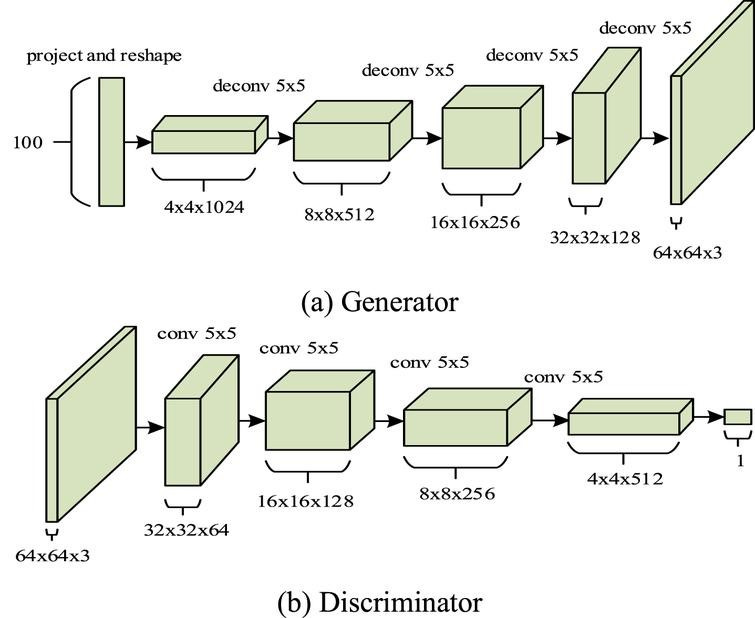
\includegraphics[width=0.7\linewidth]{Figures/dcgan.png}
    \caption{Architecture of DCGAN}
    \label{fig:dcgan}
\end{figure} 

\subsubsection*{Generator}

The generator in a DCGAN is a deep convolutional neural network designed to map a random noise vector $z \sim p_z(z) $  to a high-dimensional image space. This process can be formulated as:
\begin{equation}
    G : z \rightarrow x_{\text{fake}}
\end{equation}
where $ G(z; \theta _G) $ represents the generator network parameterized by $ \theta_G $. The network consists of a series of transposed convolutional (or deconvolutional) layers, batch normalization, and ReLU activations, except for the final layer, which often uses a Tanh activation to produce pixel values in the range $ [-1,1]$ . Mathematically, the generator optimizes the following objective function:
\begin{equation}
    \min_{\theta_G} \mathbb{E}_{z \sim p_z (z)}[log(1-D(G(z)))]
\end{equation}
where $D(G(z))$ is the probability assigned by the discriminator to the generated image being real.

\subsubsection*{Discriminator}

The discriminator is a deep convolutional neural network designed to classify whether a given image is real or synthetic. It takes an image $x$ as input and outputs a probability $ D(x) $  indicating the likelihood that the image is real. Formally, the discriminator is represented as:
\begin{equation}
    D : x \rightarrow [0,1]
\end{equation}
where $ D(x: \theta_D) $ is the discriminator network parameterized by $ \theta_D$ . The architecture consists of a series of convolutional layers with LeakyReLU activations and batch normalization, ending in a sigmoid activation function to produce a probability score. The discriminator is trained to maximize the likelihood of correctly classifying real and fake images, optimizing the following loss function:
\begin{equation}
    \max_{\theta_D} \mathbb{E}_{x \sim p_{\text{data}}(x)}[log D(x)] + \mathbb{E}_{z \sim p_z (z)}[log (1-D(G(z)))]
\end{equation}

\subsubsection*{Adversarial Training Process}

DCGAN training follows the standard GAN framework, where the generator and discriminator are trained in an adversarial manner. The overall objective function of the GAN is given by:
\begin{equation}
    \min_G \max_D V(G,D) = \mathbb{E}_{x \sim p_{\text{data}}(x)}[log D(x)] + \mathbb{E}_{z \sim p_z (z)}[log (1-D(G(z)))]
\end{equation}
This formulation defines a two-player minimax game, where the generator seeks to minimize the discriminator’s ability to distinguish real from fake images, while the discriminator seeks to maximize its classification accuracy. The training is performed iteratively, alternating between updating $ \theta_D$ and $ \theta_G $ , typically using stochastic gradient descent (SGD) or Adam optimization.

\subsection{Vision Transformers (ViTs)}

Vision Transformers (ViTs) are a novel approach to image processing that replaces traditional convolutional neural networks (CNNs) with self-attention mechanisms, initially developed for natural language processing (NLP). Unlike CNNs, which rely on hierarchical feature extraction, ViTs process images as sequences of smaller patches, allowing them to capture long-range dependencies more effectively. This section explores the architecture and working of Vision Transformers, detailing their key components and mathematical formulations \parencite{dosovitskiy2020image}. Figure \ref{fig:vit} illustrates the ViT architecture.
\begin{figure}[H]
    \centering
    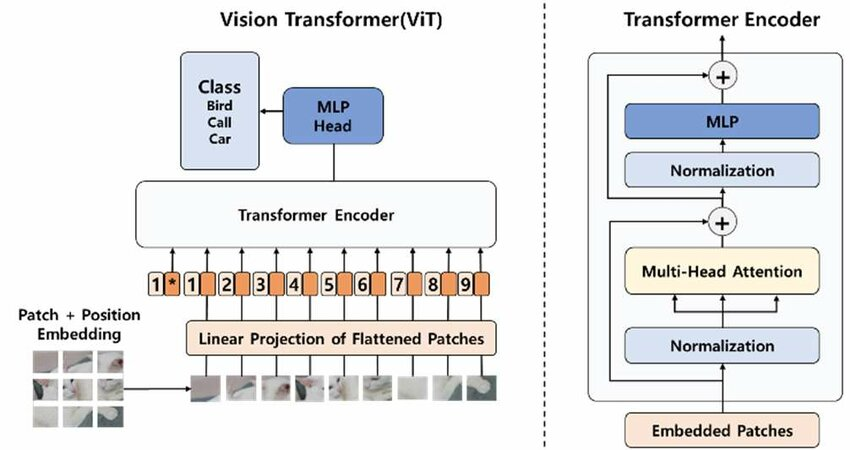
\includegraphics[width=0.7\linewidth]{Figures/vit.png}
    \caption{Architecture of ViT}
    \label{fig:vit}
\end{figure} 

\subsubsection*{Image Patch Embedding}

In ViTs, an image $ X \in  \mathbb{R}^{H \times W \times C}$ (where $H$ and $W$ are the height and width, and $C$ is the number of channels) is divided into a grid of non-overlapping patches, each of size $ P \times P$ . The number of patches, $N$ , is given by:
\begin{equation}
    N = \frac{H \times W}{P^2}
\end{equation}
Each patch is then flattened into a vector $ x_p \in \mathbb{R}^{P^2 C}$, and a trainable linear projection $E$ maps it to a lower-dimensional embedding space of size $D$. 
\begin{equation}
    z_p = Ex_p \in \mathbb{R}^D
\end{equation}
Additionally, a learnable class token $z_0$ is appended to the sequence, similar to the [CLS] token in NLP Transformers. The final input sequence $Z$ is:
\begin{equation}
    Z = [z_0 ; z_1 ; ... ; z_N] \in \mathbb{R}^{(N+1)\times D}
\end{equation}

\subsubsection*{Positional Encoding}

Since Transformers do not inherently capture spatial information, positional encodings are added to the patch embeddings. These are computed using sine and cosine functions:
\begin{equation}
    PE_{(pos,2i)} = sin \left( \frac{pos}{10000^{2i/D}} \right)
\end{equation}
\begin{equation}
    PE_{(pos,2i+1)} = cos \left( \frac{pos}{10000^{2i/D}} \right)
\end{equation}
where $pos$ is the position index, and $i$ is the embedding dimension index. These encodings are added to the patch embeddings:
\begin{equation}
    Z = Z + PE
\end{equation}

\subsubsection*{Multi-Head Self-Attention (MHSA)}

A core component of ViTs is the self-attention mechanism, which allows each token (patch) to attend to all others. Given an input sequence $Z$, three weight matrices $W_Q$ , $W_K$ , $W_V$ and  project it into query, key, and value representations:
\begin{equation}
    Q = ZW_Q \qquad K = ZW_K \qquad V = ZW_V
\end{equation}
The scaled dot-product attention is then computed as:
\begin{equation}
    Attention(Q,K,V) = softmax \left( \frac{QK^T}{\sqrt{D_k}} \right)V
\end{equation}
where $D_k$ is the dimension of the key vectors. Multi-head self-attention (MHSA) applies this mechanism in parallel using multiple heads:
\begin{equation}
    MHSA(Z) = Concat(head_1, head_2, ... , head_k)W_o
\end{equation}
where each head is computed as:
\begin{equation}
    head_i = Attention(Q_i, K_i, V_i)
\end{equation}

\subsubsection*{Feedforward Network (FFN)}

Following MHSA, each token representation passes through a Feedforward Network (FFN), consisting of two linear layers with a GELU activation function:
\begin{equation}
    FFN(x) = W_2 \cdot GELU(W_1 x+ b_1) + b_2
\end{equation}
To stabilize training, layer normalization is applied before MHSA and FFN, and residual connections are added:
\begin{equation}
    Z^{'} = Z + MHSA(LayerNorm(Z))Z^{''} = Z^{'} + FFN(LayerNorm(Z^{'}))
\end{equation}
The final output sequence $Z^{''}$  contains a special class token $z_0$, which serves as the global representation of the image. A linear classifier maps it to the final class predictions:
\begin{equation}
    \hat{y} = W_c z_0 + b_c
\end{equation}
where $W_C$ and $b_c$ are the weights and bias of the classification layer.

\section{Methodology}

\subsection{Signal Pre-processing}

Raw PSG signals often contain unwanted noise from various sources, including environmental interference, power line noise, motion artifacts, and physiological noise. To enhance signal quality, we applied a combination of low-pass filtering, high-pass filtering, and notch filtering to remove unwanted frequency components while preserving relevant information. High-Pass Filtering Used to remove slow drifts and DC components from the signals. Low-Pass Filtering applied to remove high-frequency noise and muscle artifacts.
Notch Filtering used to eliminate power line interference. Table \ref{tab:signal_specs} summarizes the specific filtering parameters used for different signal channels.

\begin{table}[H]
    \centering
    \renewcommand{\arraystretch}{0.7}
    \begin{tabular}{|c|c|c|c|c|c|}
        \hline
        \multirow{2}{*}{\textbf{Signal Type}} & \multicolumn{2}{c|}{\textbf{Value Range}} & \multicolumn{3}{c|}{\textbf{Filter Frequency}} \\
        \cline{2-6}
        & \textbf{Minimum} & \textbf{Maximum} & \textbf{High-pass} & \textbf{Low-pass} & \textbf{Notch} \\
        \hline
        EEG & -35 µV & 35 µV & 0.5 Hz & 35 Hz & 60 Hz \\
        \hline
        EOG & -35 µV & 35 µV & 0.3 Hz & 35 Hz & 60 Hz \\
        \hline
        ECG & -0.5 mV & 0.5 mV & 0.3 Hz & 70 Hz & 60 Hz \\
        \hline
        EMG & -35 µV & 35 µV & 10 Hz & 70 Hz & 60 Hz \\
        \hline
        
    \end{tabular}
    \caption{Signal specifications and filtering parameters}
    \label{tab:signal_specs}
\end{table}

\subsection{Experiment 1: Performance Evaluation of Different Image Transformation Techniques}

This experiment investigates the effectiveness of various image transformation techniques for representing PSG signals in sleep stage classification using Vision Transformers (ViTs). The transformation methods evaluated include Spectrograms, Gramian Angular Difference Field (GADF), Gramian Angular Summation Field (GASF), and Markov Transition Field (MTF). The primary objective is to determine which transformation method provides the most informative representation for Vision Transformer-based classification. \\

16 PSG channels (F7-T3, T3-T5, Fp1-F3, F3-C3, C3-P3, P3-O1, Fp2-F4, F4-C4, C4-P4, P4-O2, F8-T4, T4-T6, EOG, EMG, ECG, and Avg) were selected for this study and segmented into 30-second epochs. Each channel within an epoch was transformed into an image using the designated method. The resulting images were subsequently concatenated into a 4×4 matrix, forming a single image representation per epoch, as illustrated in Figure \ref{fig:psg_channel_img}. \\ 

A total of 12,000 epochs (with 2,000 epochs per sleep stage) were selected from the All Subjects Dataset (DS9). The pre-trained Vision Transformer (ViT-B/16) model was then fine-tuned to ensure a fair comparison across different transformation techniques.

\begin{figure}[H]
    \centering
    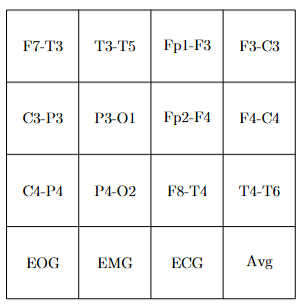
\includegraphics[width=0.5\linewidth]{Figures/psg_channels.png}
    \caption{16 PSG channels to form a unified image representation.}
    \label{fig:psg_channel_img}
\end{figure} -

\subsection{Experiment 2: Effect of Sampling Frequency and Resampling Method}

This experiment investigates the impact of different sampling frequencies and resampling methods on sleep stage classification performance. In this, 4 sampling frequencies were evaluated: 512 Hz (original), 256 Hz, 128 Hz, and 64 Hz. Additionally, two resampling methods, Fast Fourier Transform (FFT) and Discrete Wavelet Transform (DWT) were applied to determine the most effective approach. \\

Following the same approach as in Experiment 1, a total of 12,000 epochs (2,000 per sleep stage) were selected from the All Subjects Dataset (DS9). These epochs were then down-sampled to 256 Hz, 128 Hz, and 64 Hz using Fast Fourier Transform (FFT) and Discrete Wavelet Transform (DWT). The images were generated using the transformation method identified as the most effective in Experiment 1. Finally, the pre-trained Vision Transformer (ViT-B/16) model was fine-tuned to ensure a fair comparison across the different sampling frequencies and resampling methods. \\

\subsection{Experiment 3: Effectiveness of Pre-Trained vs. From-Scratch Vision Transformers}

This experiment aims to compare the performance of trained from scratch ViT models with pre-trained ViT models for sleep stage classification. Both balanced and imbalanced datasets are utilized in this experiment. \\

For this experiment, the All Subjects Dataset (DS9) was used again. Images were generated using the best methods identify in Experiments 1 and 2. The data was then used to evaluate both imbalanced and balanced datasets. To address the class imbalance, up-sampling was applied to create a balanced dataset. Once both balanced and imbalanced datasets were prepared, the ViT model was first trained from scratch and tuned to achieve the best performance. Subsequently, the pre-trained ViT-B/16 model was fine-tuned for both datasets.

\subsection{Experiment 4: Effectiveness of Different Pre-Trained Vision Transformers}

Given that fine-tuning the ViT-B/16 model outperformed training from scratch, further experiments have to conduct to compare the performance of various pre-trained ViT models. The aim was to identify the model that provides the best classification accuracy while ensuring optimal computational efficiency. \\

Based on the results from Experiments 1 and 2, a balanced image dataset was created using the DS9 dataset. The following pre-trained ViT models were then fine-tuned on this dataset: ViT-B/32, DeiT-B, Swin-B, BEiT-B, and PVT-Small.

\subsection{Experiment 5: Training and Tuning DCGAN for Synthetic Image Generation}

To address the challenges of subject-to-subject variability and class imbalances in sleep stage classification, GAN-based data augmentation was employed. The primary objective was to enhance the diversity of training samples, thereby improving model generalization. Specifically, a Deep Convolutional Generative Adversarial Network (DCGAN) was implemented to generate realistic synthetic data, contributing to a more balanced and representative training set. \\

First, images for the DS9 dataset were generated based on the results from Experiments 1 and 2. The dataset was then split into 70\% for training and 30\% for validation. Subsequently, various architectures DCGANs were trained and tuned to generate synthetic PSG images.

\subsection{Experiment 6: Effectiveness of GAN-Augmented Data}

In Experiment 5, the primary objective was to train a DCGAN model for the generation of synthetic PSG image representations. The focus of this experiment was to evaluate the effectiveness of the generated synthetic data in improving sleep stage classification performance. \\

First, images for the DS9 dataset are generated based on the results from Experiments 1 and 2. These images are then separated according to the corresponding sleep stages. Next, the trained DCGAN model is fine-tuned for each sleep stage class, generating 20,000 synthetic images per class. \\

Following this, the best-performing classification model identified after Experiment 4 is selected. This model is then fine-tuned on three different datasets:
\begin{enumerate}
    \item The \textbf{original dataset} (with upsampling applied only in this case)
    \item The \textbf{GAN-augmented dataset} (containing only synthetic images)
    \item A \textbf{mixed dataset} (comprising both original and synthetic images)
\end{enumerate}
For each dataset, 10,000 images per class randomly used for training.

\subsection{Final Model Selection}

Following Experiment 6, the best-performing model is identified as the optimal model for this study. After selecting this model, its performance is further evaluated on DS1–DS8 datasets to assess its generalization capability across different data distributions.\\

\begin{figure}[H]
    \centering
    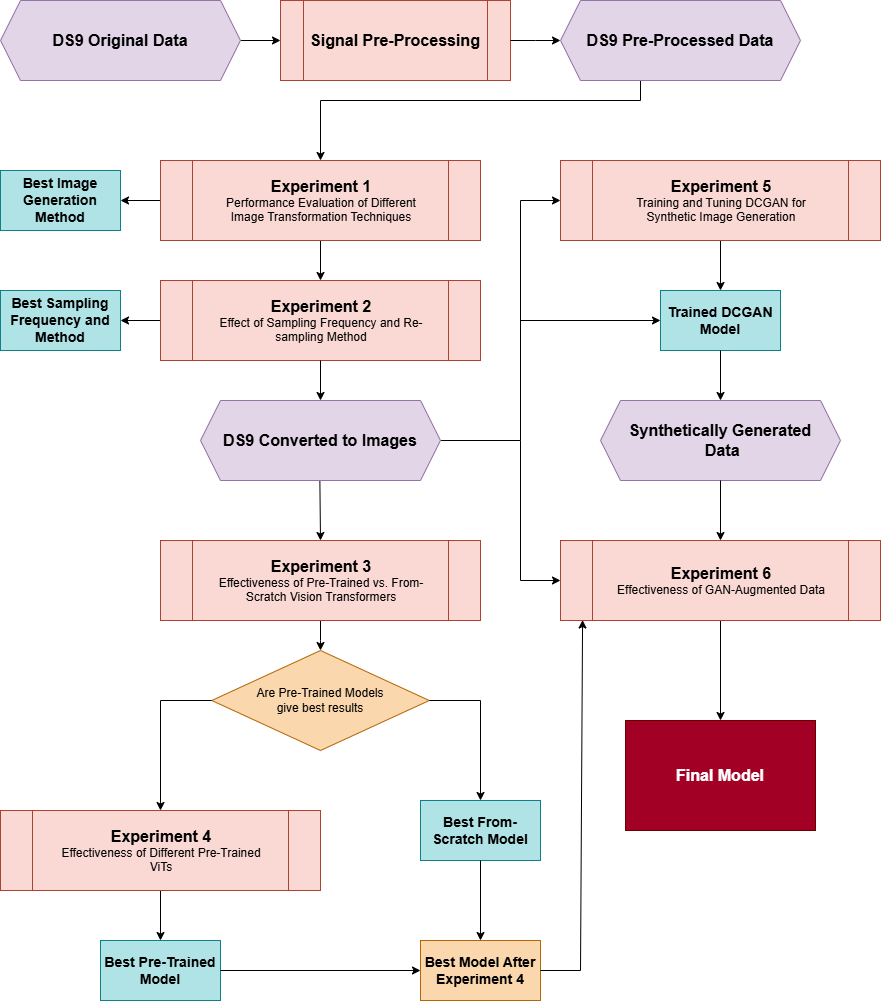
\includegraphics[width=1\linewidth]{Figures/methodology.png}
    \caption{Overview of Methodology}
    \label{fig:methodology_overview}
\end{figure} 


\chapter{Data}


\section{CAP Sleep Database}

The EEG dataset used in this study was obtained from PhysioNet’s publicly available CAP Sleep Database \parencite{goldberger2000physiobank}. The sleep scoring was conducted by a team of experts from the Sleep Disorders Centre at Ospedale Maggiore in Parma, Italy.. \\

The CAP Sleep Database comprises 108 PSG recordings, all collected at the same medical center. These recordings include multiple physiological signals, such as at least three EEG channels C3 or C4, F3 or F4, and O1 or O2 referenced to A1 or A2. Additionally, the dataset contains EOG channels, submental muscle EMG, respiration signals, bilateral tibial EMG, and one EKG. The EEG recordings also include bipolar configurations such as F3-C3, Fp1-F3, P3-O1, C3-P3, C4-P4, Fp2-F4, P4-O2, and F4-C4. \\

To provide a visual reference of the dataset's structure and signal characteristics, Figure \ref{fig:physionet} presents a 10-second snapshot of PSG data from a single subject, illustrating the morphology and quality of signals across multiple channels.

\begin{figure}[H]
    \centering
    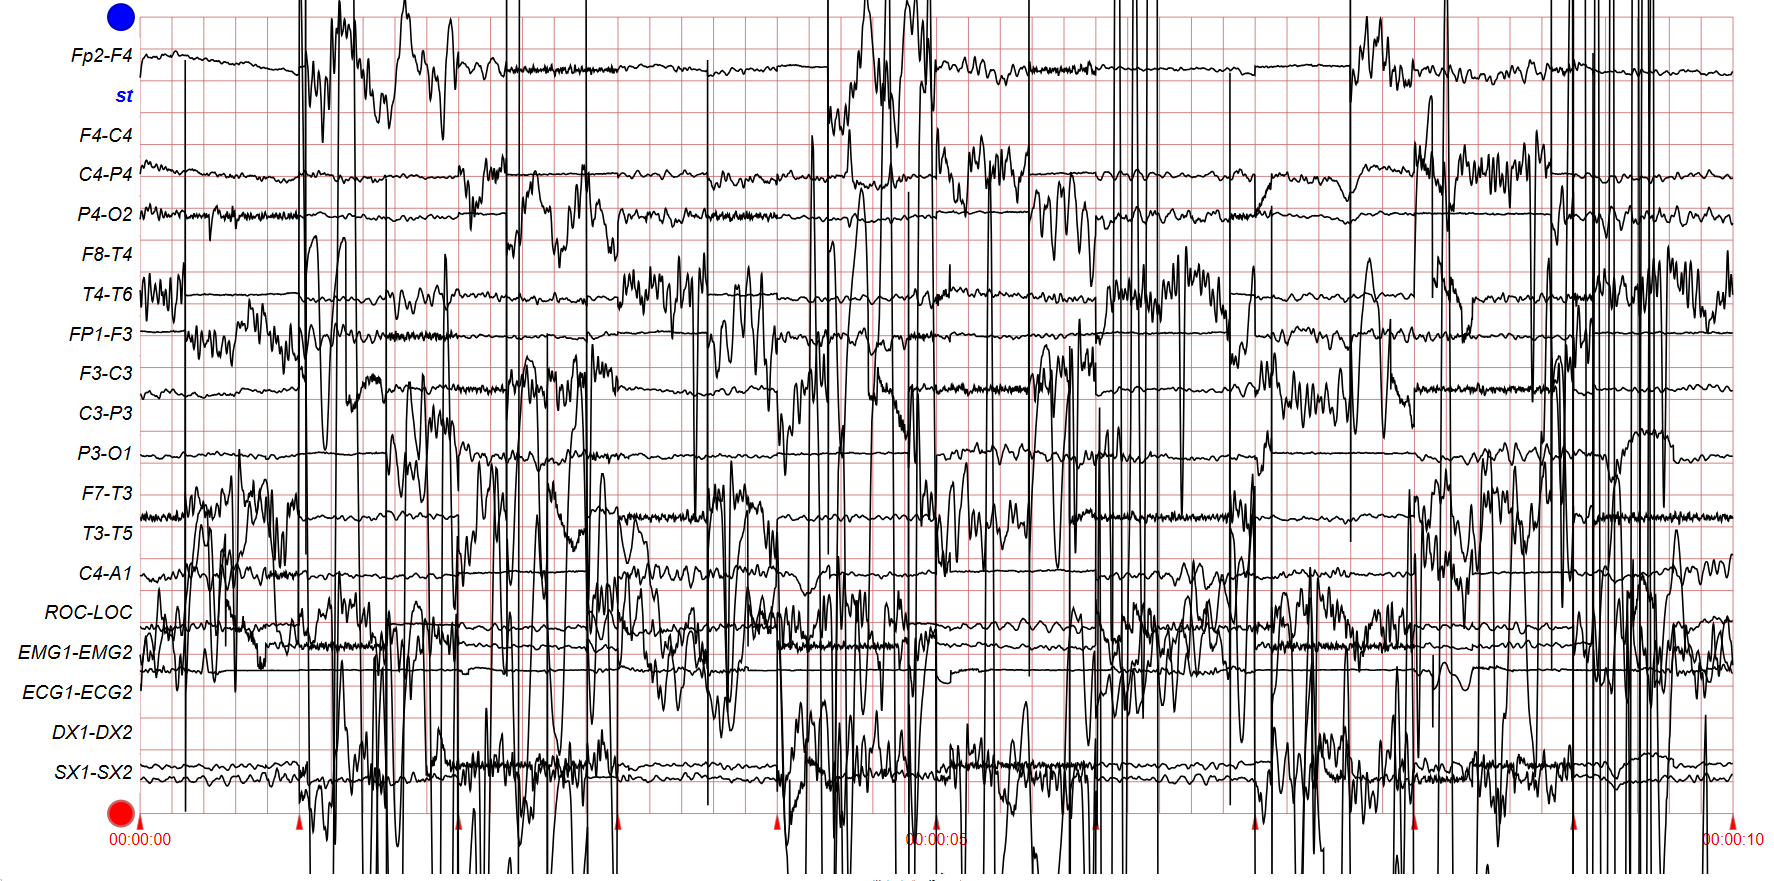
\includegraphics[width=1\linewidth]{Figures/physionet.png}
    \caption{10-second PSG segment from one subject in the CAP Sleep Database}
    \label{fig:physionet}
\end{figure}

The EEG recordings in the dataset were collected at varying sampling frequencies, ranging from 100 Hz to 512 Hz, and vary in duration from approximately 2 to 9 hours. For the purpose of sleep stage classification, the data was segmented into \textbf{epochs} (fixed length time windows of 30 seconds), which serve as the standard unit of analysis in sleep research. \\

Sleep scoring was performed by trained experts following the Rechtschaffen \& Kales (R\&K) guidelines. Each epoch was labeled with a corresponding sleep stage: W for wakefulness, S1–S4 for non-REM (NREM) stages, and R for Rapid Eye Movement (REM) sleep. \\

The dataset includes recordings from both healthy individuals and patients diagnosed with seven different sleep disorders, namely Insomnia, Bruxism, Narcolepsy, Nocturnal Frontal Lobe Epilepsy (NFLE), Periodic Leg Movement (PLM), REM Behavior Disorder (RBD), and Sleep-Disordered Breathing (SDB).  Among the 108 subjects, 16 are completely healthy, while the remaining 92 participants are diagnosed with sleep disorders. 40 have NFLE, 22 experience RBD, 10 have PLM, 9 suffer from insomnia, 5 are diagnosed with narcolepsy, 4 have sleep-disordered breathing, and 2 are affected by bruxism. \\

The participants' ages range from 14 to 82 years, with an average age of approximately 45 years. The dataset consists of 61\% male participants (66 individuals) and 38\% female participants (42 individuals). A summary of these demographic and diagnostic details is presented in Table \ref{tab:cap_sleep}.\\

\begin{table}[H]
    \centering
    \small % Reduce font size to 10pt
    \resizebox{0.6\textwidth}{!}{ % Adjust width
    \begin{tabular}{lccc}
        \toprule
        \textbf{Subject Type} & \textbf{N} & \textbf{M/F} & \textbf{Age (Mean ± SD)} \\
        \midrule
        Healthy    & 16  & 7/9  & 32.19 ± 5.55  \\
        Insomnia   & 9   & 4/5  & 60.89 ± 10.53  \\
        Bruxism    & 2   & 2/0  & 28.5 ± 7.78  \\
        Narcolepsy & 5   & 2/3  & 31.6 ± 11.55  \\
        NFLE       & 40  & 21/19  & 30.28 ± 10.89  \\
        PLM        & 10  & 7/3  & 55.10 ± 6.71  \\
        RBD        & 22  & 19/3  & 70.72 ± 6.37  \\
        SBD        & 4   & 4/0  & 71.25 ± 7.23  \\
        \midrule
        \textbf{Total} & 108  & 66/42 & \textbf{45.19 ± 19.56} \\
        \bottomrule
    \end{tabular}
    }
    \caption{Summary of CAP Sleep Database}
    \label{tab:cap_sleep}
\end{table}


Despite the rich data available in the CAP Sleep Database, most existing studies focus on cyclic phase detection rather than sleep stage classification. While many datasets have been used for sleep stage detection, only few research has specifically utilized the CAP Sleep Database for this purpose.

\section{Data Acquisition for Research}
Subjects  whom had EEG recordings sampled at 512 Hz were selected for this study. 80 subjects, including 6 healthy individuals and 74 individuals with sleep disorders were selected accordingly. Further details for selected subjects on the total number of epochs for each sleep stage across different patient groups are provided in Table \ref{tab:sleep_stages}. Each row in the table corresponds to a specific sleep stage Wake, S1, S2, S3, S4, and REM while each column represents the number of 30 second epochs recorded for that stage across different subject groups. The final two columns summarize the total number of epochs per sleep stage and their corresponding percentage relative to the overall dataset \\

\begin{table}[H]
    \centering
    \resizebox{\textwidth}{!}{ 
    \begin{tabular}{l | r  r r r r r r r | r r} 
        \toprule
        
        Sleep Stage & Healthy & Insomnia & Bruxism & Narcolepsy & NFLE & PLM & RBD & SBD & Total &  (\%) \\
        \midrule
        Wake & 445 & 3801 & 44 & 1303 & 3155 & 1332 & 5266 & 495 & 15841 & 19.64\% \\
        S1   & 280 & 223  & 34  & 301  & 1098 & 266  & 1048  & 269 & 3519  & 4.36\% \\
        S2   & 2172 & 2456 & 144 & 1708 & 10630 & 2748 & 7486 & 1324 & 28628 & 35.50\% \\
        S3   & 573 & 670  & 39  & 476  & 2987  & 955  & 2880  & 224  & 8804  & 10.92\% \\
        S4   & 1184 & 415  & 99  & 568  & 4108  & 956  & 2506  & 352  & 10188 & 12.63\% \\
        REM  & 1409 & 986  & 67  & 1258 & 4905  & 1317 & 3530  & 215  & 13687 & 16.97\% \\
        \midrule
        Total & 6063 & 8551 & 427 & 5614 & 26883 & 7574 & 22676 & 2879 & \textbf{80667} & \textbf{100\%}\\
        \bottomrule
    \end{tabular}
    } % End of resizebox
    \caption{Sleep stage wise details of epoch distribution for selected subjects}
    \label{tab:sleep_stages}
\end{table}


Then created 9 distinct data subsets, namely: Healthy, Insomnia, Bruxism, Narcolepsy, NFLE, PLM, RBD, SDB, and All Subjects Combined. Sleep stage classification was performed separately on each subset. \\

For each data subset, a detailed description of each subset is provided below:

\begin{enumerate}
    \item \textbf{Healthy (DS1):} This subset includes sleep stage epochs from individuals with no reported sleep disorders. It consists of 6 healthy subjects, with a total of 6,063 epochs.
    
    \item \textbf{Insomnia (DS2):} This subset contains sleep stage epochs from 7 individuals diagnosed with insomnia, totaling 8,551 epochs. 
    
    \item \textbf{Bruxism (DS3):} This dataset includes 427 epochs from 1 individual affected by bruxism sleep disorder. 
    
    \item \textbf{Narcolepsy (DS4):} It consists of data from 5 individuals, comprising 5,614 epochs.
    
    \item \textbf{NFLE (DS5):} This subset includes 26,883 epochs from 27 individuals diagnosed with nocturnal frontal lobe epilepsy (NFLE). 
    
    \item \textbf{PLM (Periodic Leg Movement Disorder) (DS6):} It contains 7,574 epochs obtained from 9 individuals with PLM. 

    \item \textbf{RBD (REM Behavior Disorder) (DS7):} This dataset comprises 22,676 epochs collected from 22 individuals diagnosed with RBD. 

    \item \textbf{SDB (Sleep-Disordered Breathing) (DS8):} It includes 2,879 epochs from 3 individuals diagnosed with SDB. 

    \item \textbf{All Subjects Combined (DS9):} This dataset includes data from all 80 subjects, encompassing both healthy and disordered individuals, with a total of 80,667 epochs. 
    
\end{enumerate}

Each PSG recording contained several types signals. We have only used EEG, EOG, ECG and EMG channels for this study.






\chapter{Preliminary Analysis}

In this section, we provide an in-depth analysis of the EEG data used in the study, focusing on artifact detection and inter-subject variations. These factors are critical to the quality of the EEG signals and directly impact the performance of sleep stage classification models.

\section{Artifact Detection}

EEG data is often contaminated by various artifacts that can interfere with the accurate interpretation of brain activity, particularly in the context of sleep stage classification. This analysis focuses on identifying common types of artifacts, including power line noise, cardiac signal noise, eye movement artifacts, and bad channel noise. These artifacts were identified using diagnostic techniques such as power spectrogram analysis and Independent Component Analysis (ICA), with supporting visualizations provided through graphs and diagnostic plots. \\

In Figure \ref{fig:powerlinenoise}, the power spectrogram for a randomly selected subject clearly shows a distinct spike at 60 Hz, which is indicative of power line noise. This periodic interference is commonly caused by the electrical power grid, which introduces noise at this frequency. Additionally, smaller spikes are observed around multiples of 15 Hz, which can be attributed to cardiac signal noise. This noise results from the electrical activity of the heart, which often contaminates the EEG signal, especially in the low-frequency range. These observations highlight the presence of both power line and cardiac signal artifacts in the EEG data, necessitating appropriate artifact removal techniques for accurate analysis.

\begin{figure}[H]
    \centering
    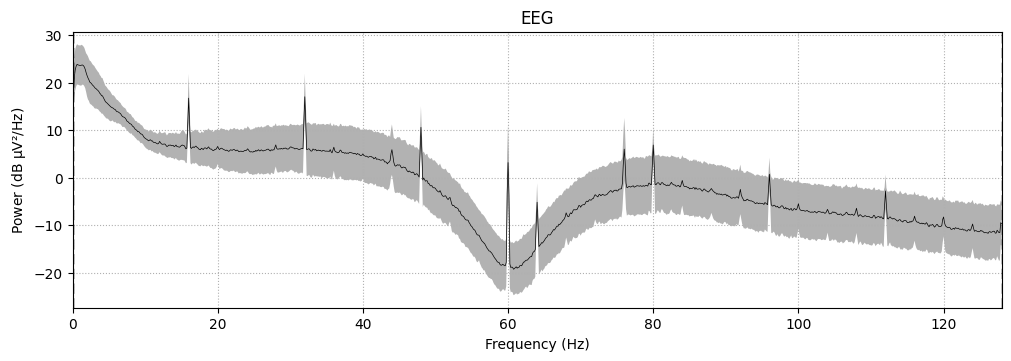
\includegraphics[width=1\linewidth]{Figures/powerlinenoise.png}
    \caption{Power spectrogram showing power line noise and cardiac signal noise of a randomly selected subject.}
    \label{fig:powerlinenoise}
\end{figure} 

In Figure \ref{fig:ica}, the topographic maps for each ICA component of a randomly selected subject are presented. Two components, ICA000 and ICA019, are identified as corresponding to specific artifacts. ICA000 is associated with eye movement artifacts, as evidenced by signal saturation near the eye region. Similarly, ICA019 is linked to a bad channel, with signal saturation localized to a single area. These findings are crucial for identifying and isolating artifacts in the EEG data for further analysis.

\begin{figure}[H]
    \centering
    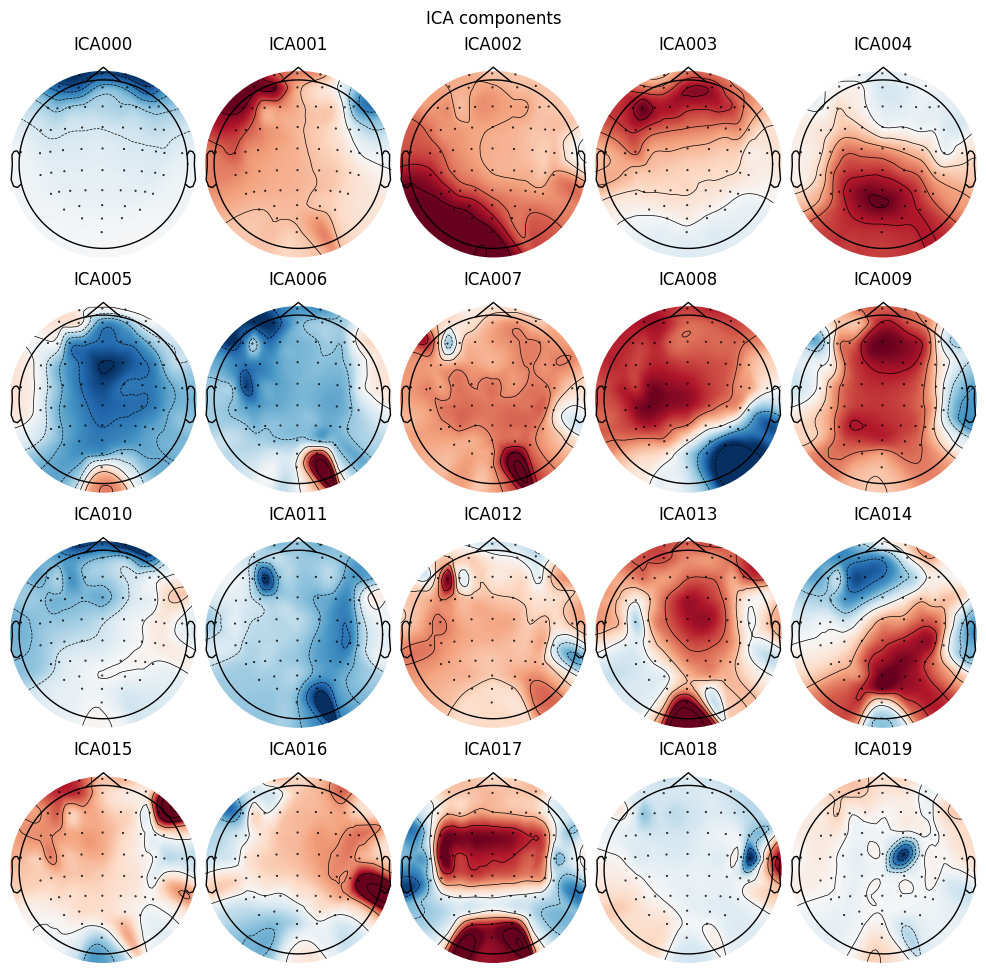
\includegraphics[width=0.6\linewidth]{Figures/ica.png}
    \caption{Topographic maps for ICA components of a randomly selected subject.}
    \label{fig:ica}
\end{figure} 

By eliminating these artifacts, the quality of the data is significantly improved. Hence removal of artifacts through signal preprocessing is essential for ensuring the accuracy and reliability of EEG data in sleep stage classification. 

\section{Inter Subject Variations in EEG}

Inter-subject variations are differences in EEG signals that arise between different individuals. These variations can be attributed to numerous factors, including individual differences in brain structure, electrode placement, and physiological responses during sleep. Inter-subject variability is one of the most significant challenges in EEG-based sleep stage classification, as it can make it difficult for models trained on one subject’s data to generalize effectively to others. \\

Figure \ref{fig:s_power} presents the power spectrograms of three randomly selected subjects for their S3 sleep stage. It is evident that the spectrograms exhibit distinct patterns for each subject, reflecting variations in the EEG signal characteristics. These differences highlight the individual variability in the brain’s electrical activity during sleep, which must be accounted for in analysis and model training to ensure generalization across subjects. \\

Further, Figure \ref{fig:connectivity} presents the connectivity matrices of EEG electrodes for two randomly selected subjects during the same sleep stage (S3). The matrices reveal noticeable differences in electrode connectivity between the subjects. This variability further emphasizes the need for handle inter-subject differences effectively. Recognizing and addressing such variations is crucial for improving the performance of sleep stage classification models, as it helps ensure that the model generalizes well across diverse data sources. \\ 

By understanding and addressing inter-subject variability in EEG data, the accuracy and reliability of sleep stage classification can be improved, ultimately leading to more effective and personalized analyses.

\begin{figure}[H]
    \centering
    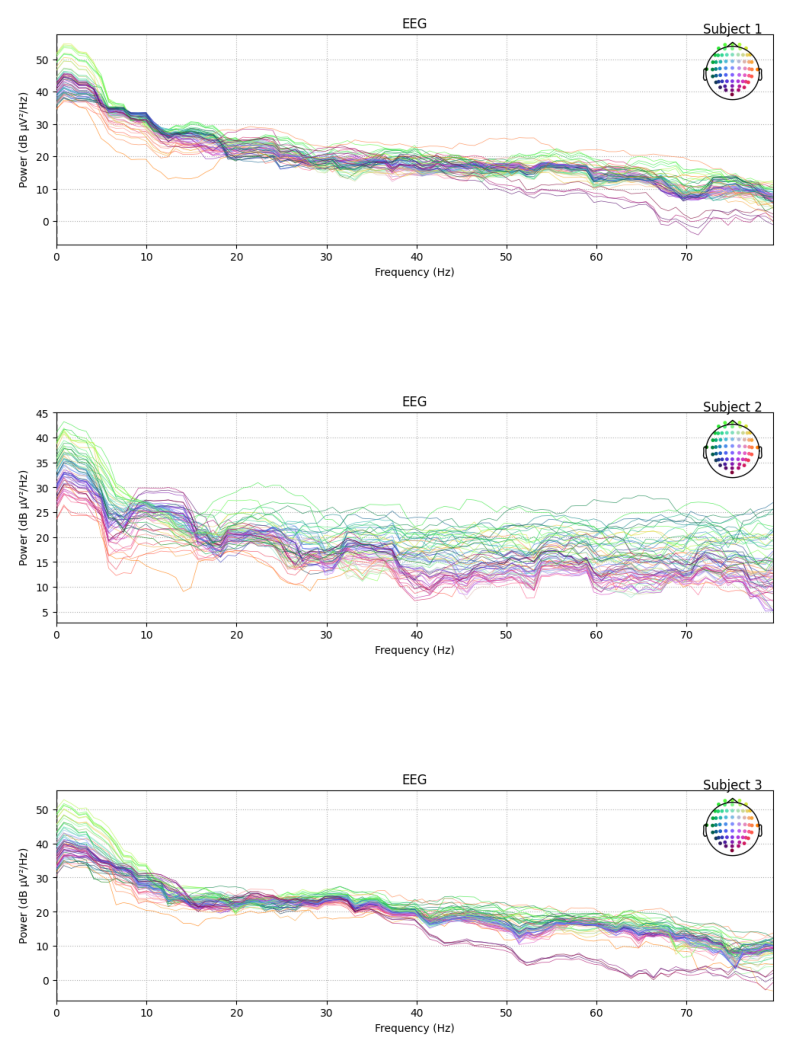
\includegraphics[width=0.65\linewidth]{Figures/s_power.png}
    \caption{Power spectrograms for three randomly selected subjects showing distinct EEG signal patterns across S3 sleep stage.}
    \label{fig:s_power}
\end{figure}

\begin{figure}[H]
    \centering
    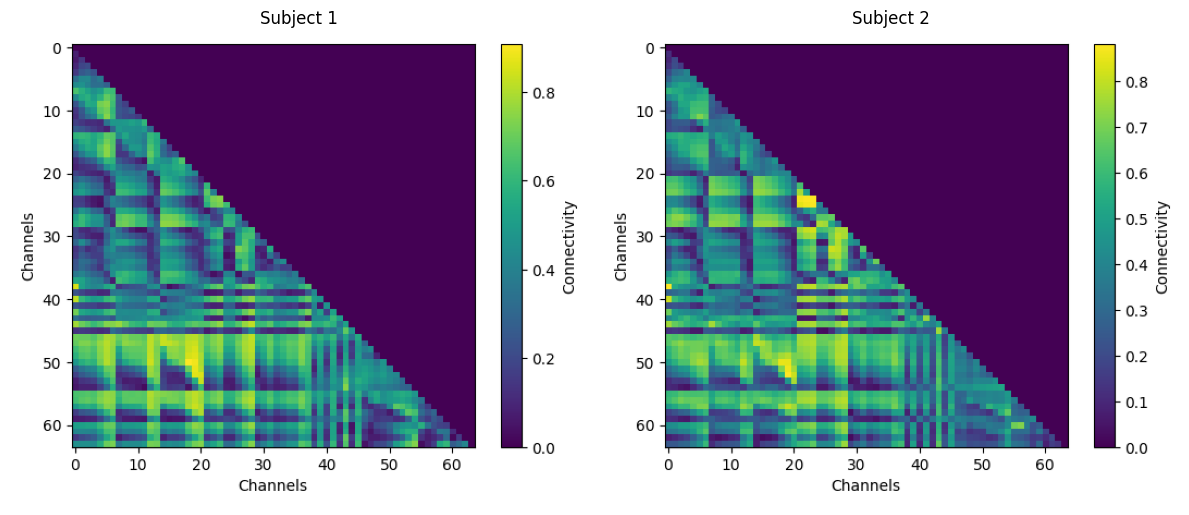
\includegraphics[width=1\linewidth]{Figures/connectivity.png}
    \caption{Connectivity matrices for two randomly selected subjects during the S3 sleep stage.}
    \label{fig:connectivity}
\end{figure}



\chapter{Results and Discussion}

\section{Performance Evaluation of Different Image Transformation Techniques}

This section presents the findings of the experiment evaluating four image transformation techniques Spectrograms, GADF, GASF, and MTF for sleep stage classification using Vision Transformers. Figure \ref{fig:ts2img} provides a visual comparison of these methods applied to the same epoch. The classification performance was summarized in Table \ref{tab:transformation_methods_performences}. These findings offer insights into the most effective transformation method for PSG signal representation in Vision Transformer-based sleep stage classification.

\begin{figure}[H]
    \centering
    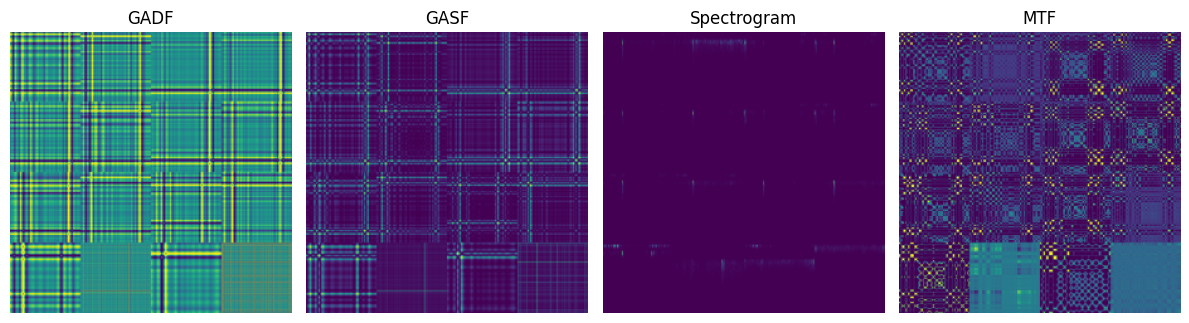
\includegraphics[width=1\linewidth]{Figures/ts2img.png}
    \caption{Visual representation of different image transformation techniques applied to sleep stage classification.}
    \label{fig:ts2img}
\end{figure} 

\begin{table}[H]
    \centering
    \resizebox{\textwidth}{!}{%
    \begin{tabular}{lcccc}
        \toprule
        \textbf{Transformation Method} & \textbf{Accuracy (\%)} & \textbf{F1-Score} & \textbf{Processing Time (s/epoch)} \\
        \midrule
        Spectrogram & 55.4 & 0.54  & 0.4 \\
        GADF        & 56.7 & 0.55  & 0.2 \\
        GASF        & 57.2 & 0.57  & 0.2 \\
        MTF         & 57.1 & 0.56  & 5 \\
        \bottomrule
    \end{tabular}%
    }
    \caption{Performance comparison of image transformation techniques for sleep stage classification.}
    \label{tab:transformation_methods_performences}
\end{table}

Among the tested methods, GASF achieved the highest accuracy (57.2\%) and F1-score (0.57), making it the most informative representation for the ViT-based classifier. MTF showed comparable accuracy (57.1\%) and F1-score (0.56), but its high processing time (5 seconds per epoch) makes it impractical for large-scale applications. GADF demonstrated moderate performance (Accuracy: 56.7\%, F1-score: 0.55) but was computationally efficient, requiring only 0.2 seconds per epoch. Spectrograms performed the worst (Accuracy: 55.4\%, F1-score: 0.54), indicating weak feature representation for ViT. \\

Overall, GASF is the most effective transformation, offering a balance between high classification performance and computational efficiency. While MTF provides similar accuracy, its high processing time limits its real-time usability. \\ 

To further assess each transformation technique, feature embeddings from the final layer of ViT-B/16 were extracted and visualized using t-Distributed Stochastic Neighbor Embedding (t-SNE). Figure \ref{fig:tsne_img} illustrates the t-SNE plots for all four methods. The t-SNE visualizations did not reveal clearly separable clusters, suggesting that t-SNE alone is insufficient for evaluating transformation distinctiveness. Therefore, clustering quality was assessed using Silhouette Score, Davies-Bouldin Index (DBI), and Calinski-Harabasz Index (CHI) (Table \ref{tab:transformation_methods_cluster_performences}). 

\begin{figure}[H]
    \centering
    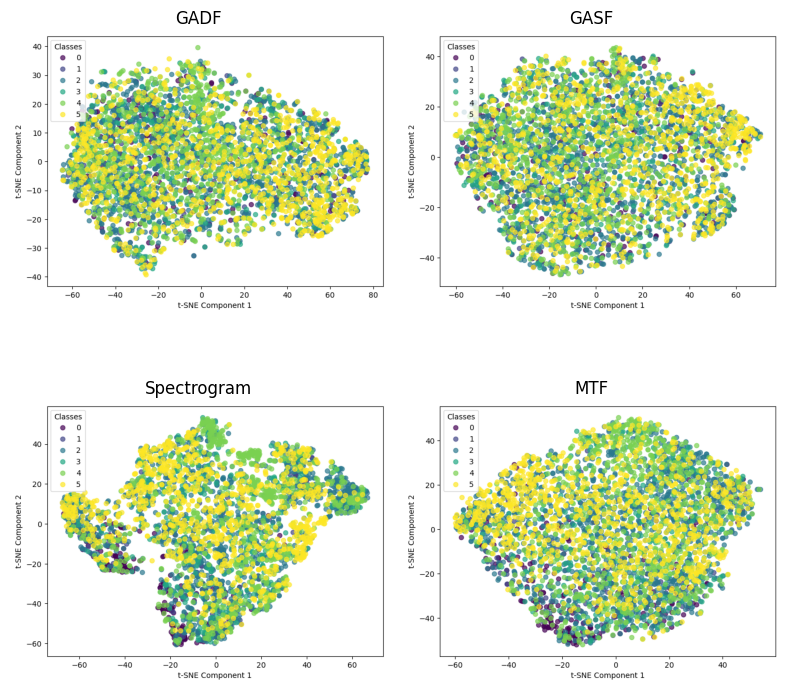
\includegraphics[width=0.8\linewidth]{Figures/tsne.png}
    \caption{t-SNE visualization of feature embeddings extracted from the ViT-B/16 for the GADF, GASF, Spectrogram, and MTF.}
    \label{fig:tsne_img}
\end{figure}

\begin{table}[H]
    \centering
    \resizebox{\textwidth}{!}{%
    \begin{tabular}{lcccc}
        \toprule
        \textbf{Transformation} & \textbf{Silhouette} & \textbf{Davies-Bouldin} & \textbf{Calinski-Harabasz}\\

        \textbf{Method} & \textbf{Score} & \textbf{Index} & \textbf{Index}\\
        \midrule
        Spectrogram & -0.05 & 45.44 & 20.41 \\
        GADF        & -0.07 & 10.51 & 49.70 \\
        GASF        & -0.08 & 10.45 & 53.79 \\
        MTF         & -0.07 & 23.88 & 19.76 \\
        \bottomrule
    \end{tabular}%
    }
    \caption{Clustering Performance for Different Image Transformations}
    \label{tab:transformation_methods_cluster_performences}
\end{table}

The Silhouette Score was negative for all methods, indicating poor clustering. Spectrograms had the highest score (-0.05), while GASF had the lowest (-0.08), suggesting weak cluster separability. The DBI showed that GASF (10.45) and GADF (10.51) achieved the best cluster separation, whereas Spectrograms (45.44) and MTF (23.88) exhibited substantial overlap. The CHI further confirmed GASF as the best method (53.79), followed by GADF (49.70), while Spectrograms (20.41) and MTF (19.76) demonstrated poor clustering performance. \\

Overall, GASF and GADF produced more structured and distinct clusters, making them better feature representations for sleep stage classification. Spectrograms and MTF exhibited weak clustering, aligning with the t-SNE findings. \\

Therefore, among the evaluated image transformation techniques, GASF emerged as the most effective, balancing high classification performance, computational efficiency, and structured feature representation. 


\section{Effect of Sampling Frequency and Resampling Method}

This section presents the findings on the impact of sampling frequency and resampling methods on sleep stage classification performance. Classification accuracy was evaluated across four sampling frequencies (512 Hz, 256 Hz, 128 Hz, and 64 Hz) and two resampling methods (FFT and DWT) to determine the most effective combination. Based on the results of Experiment 1, GADF was selected as the image transformation method. Figures \ref{fig:fft_img} and \ref{fig:dwt_img} visually represent the resampling methods at different frequencies applied to the same epoch. The results, summarized in Table \ref{tab:effect_of_frequency}, provide insights into how downsampling and resampling influence PSG signal representation for Vision Transformer-based classification.
\begin{figure}[H]
    \centering
    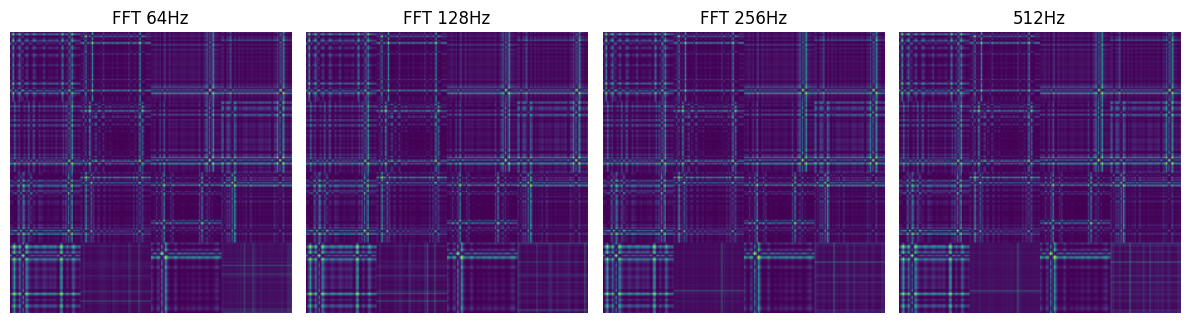
\includegraphics[width=1\linewidth]{Figures/fft.png}
    \caption{GASF representations at different sampling frequencies using Fast Fourier Transform.}
    \label{fig:fft_img}
\end{figure}

\begin{figure}[H]
    \centering
    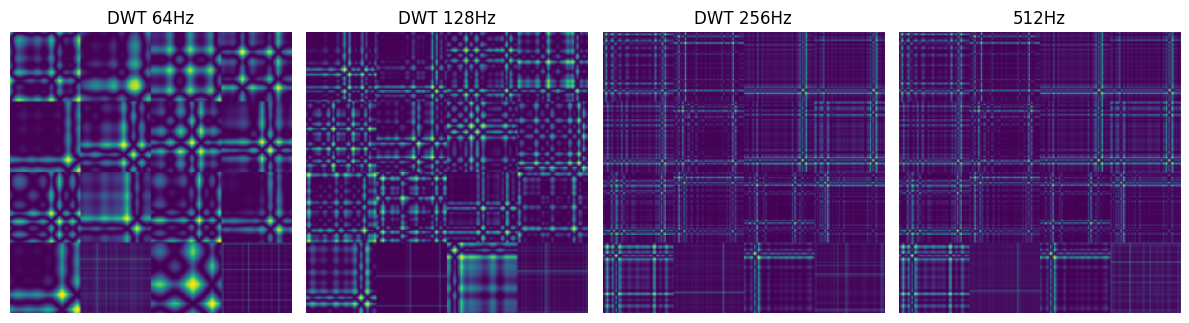
\includegraphics[width=1\linewidth]{Figures/dwt.png}
    \caption{GASF representations at different sampling frequencies using Discrete Wavelet Transform.}
    \label{fig:dwt_img}
\end{figure}

\begin{table}[H]
    \centering
    \resizebox{\textwidth}{!}{ % Resize to fit within page width
    \begin{tabular}{llcccc}
        \toprule
        \textbf{Sampling Frequency} & \textbf{Resampling Method} & \textbf{Accuracy (\%)} & \textbf{F1-Score} \\
        \midrule
        512 Hz & Original  & 57.2 & 0.57   \\
        256 Hz & FFT  & 58.0 & 0.57   \\
        256 Hz & DWT  & 58.5 & 0.58   \\
        128 Hz & FFT  & 56.3 & 0.55  \\
        128 Hz & DWT  & 60.1 & 0.60   \\
        64 Hz  & FFT  & 53.8 & 0.52   \\
        64 Hz  & DWT  & 56.4 & 0.56   \\
        \bottomrule
    \end{tabular}
    }
    \caption{Performance of sleep stage classification using different sampling frequencies and resampling methods.}
    \label{tab:effect_of_frequency}
\end{table}

The results indicate that down-sampling using DWT at 128 Hz achieved the highest performance, with an accuracy of 60.1\% and an F1-score of 0.60. This suggests that the combination of lower sampling frequency and the DWT resampling method enhances the model's ability to classify sleep stages accurately. Notably, DWT at 256 Hz also showed strong performance, with an accuracy of 58.5\% and an F1-score of 0.58, indicating that DWT offers better results compared to FFT for similar sampling frequencies. \\

In contrast, the FFT method at 128 Hz resulted in a lower accuracy of 56.3\% and F1-score of 0.55, suggesting that FFT may be less effective at lower sampling frequencies. Furthermore, the performance at 64 Hz was significantly lower, with an accuracy of 53.8\% and an F1-score of 0.52, particularly when using FFT. Even with the DWT method at 64 Hz, the performance was still lower (56.4\% accuracy, 0.56 F1-score), further highlighting the challenges of downsampling to very low frequencies. \\

Interestingly, the original 512 Hz data (without downsampling) achieved an accuracy of 57.2\% and an F1-score of 0.57, showing that while downsampling improves computational efficiency, it may come at the cost of classification accuracy—especially when using FFT. \\

Overall, the results suggest that DWT resampling provides the best trade-off between classification accuracy and computational efficiency, especially at 128 Hz and 256 Hz. FFT, on the other hand, tends to perform less effectively at lower sampling frequencies, especially when downsampling to 64 Hz.



\section{Effectiveness of Pre-Trained vs. From-Scratch ViTs}

This section presents the findings on the effectiveness of pre-trained versus from-scratch Vision Transformers (ViTs) for sleep stage classification. The experiments were conducted using both balanced and imbalanced datasets to evaluate the models’ generalization capabilities. Based on prior experiments, the Gramian Angular Summation Field (GASF) with Discrete Wavelet Transform (DWT) at 128 Hz was selected as the optimal image transformation method. \\ 

The from-scratch ViT model was developed after experimenting with various architectures and hyperparameter tuning to optimize sleep stage classification performance. Different configurations of embedding dimensions, attention heads, and transformer layers were explored to balance model complexity and generalization. The final architecture is summarized in Table \ref{tab:best_from_scratch}. \\

\begin{table}[H]
    \centering
    \begin{tabular}{l c}
        \toprule
        \textbf{Component} & \textbf{Details} \\
        \midrule
        Patch Size & 16 × 16 \\
        Embedding Dimension (D) & 256 \\
        Transformer Layers (L) & 6 \\
        Attention Heads & 8 \\
        MLP Hidden Dimension & 512 \\
        Dropout & 0.1 \\
        Classifier Head & Fully Connected (FC) + Softmax \\
        \bottomrule
    \end{tabular}
    \caption{ Summary of the Best Performing From-Scratch ViT Architecture}
    \label{tab:best_from_scratch}
\end{table}

Figure \ref{fig:fn_scrtach} illustrates the results, showing a clear performance advantage of the pre-trained ViT over the from-scratch model. The pre-trained ViT achieved a 78.1\% accuracy on the balanced dataset, outperforming the from-scratch ViT by 9.2\%. Similarly, for the imbalanced dataset, the pre-trained ViT obtained 68.5\% accuracy, which is 4.1\% higher than the from-scratch model.

\begin{figure}[H]
    \centering
    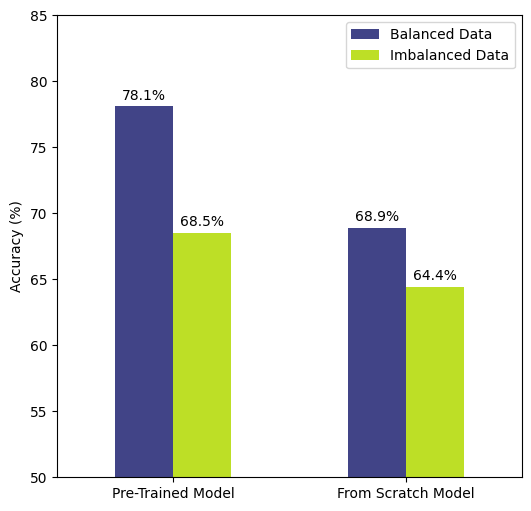
\includegraphics[width=0.6\linewidth]{Figures/fn_scratch.png}
    \caption{Comparison of Accuracy for Fine-Tuned and Model from Scratch on Balanced and Unbalanced Data}
    \label{fig:fn_scrtach}
\end{figure}

These results suggest that leveraging transfer learning with a pre-trained ViT significantly enhances classification accuracy, especially when data availability is limited or imbalanced. The superior performance of the pre-trained model highlights the benefits of prior feature extraction from large-scale datasets, enabling better generalization to sleep stage classification.

\section{Effectiveness of Different Pre-Trained Vision Transformers}

This section presents the findings on the effectiveness of different pre-trained Vision Transformer models for sleep stage classification. Building on previous experiments, a balanced image dataset was created using the DS9 dataset, and multiple pre-trained ViT models—ViT-B/16, ViT-B/32, DeiT-B, Swin-B, BEiT-B, and PVT-Small—were fine-tuned using a consistent preprocessing pipeline. The results, summarized in Table \ref{tab:pre_trained_models} and Figure \ref{fig:pretrained_models}, provide insights into the classification performance and computational efficiency of each model, helping identify the most suitable ViT architecture for sleep stage classification.

\begin{table}[H]
    \centering
    \resizebox{\textwidth}{!}{ % Resize to fit within page width
    \begin{tabular}{llcccc}
        \toprule
        \textbf{Model} & \textbf{Accuracy (\%)} & \textbf{F1-Score} & \textbf{Inference Time (ms/eppoch)} \\
        \midrule
        ViT-B/16 & 78.1  & 77.2 & 290   \\
        ViT-B/32 & 75.8  & 73.9 & 320   \\
        DeiT-B	 & 76.4  & 74.5 & 250   \\
        Swin-B	 & 77.9  & 76.1 & 280  \\
        BEiT-B	 & 77.2  & 75.5 & 330   \\
        PVT-Small & 73.8  & 71..9 & 200   \\
        \bottomrule
    \end{tabular}
    }
    \caption{Performances of Pre trained models}
    \label{tab:pre_trained_models}
\end{table}

The evaluation focused on key performance metrics, including accuracy, F1-score, and inference time per epoch. The results indicated that ViT-B/16 achieved the highest classification accuracy of 78.1\%, followed closely by Swin-B at 77.9\%. ViT-B/16 also recorded the highest F1-score of 77.2\%, reinforcing its superior ability to capture sleep stage patterns effectively. In contrast, ViT-B/32, a variant with a larger patch size, exhibited slightly lower accuracy at 75.8\%, which suggests that smaller patch sizes may be more effective in extracting fine-grained details from PSG-based image representations. The BEiT-B model achieved 77.2\% accuracy, which was slightly lower than Swin-B, indicating that masked image modeling-based pre-training does not significantly improve sleep stage classification in this setting. \\

Among the models tested, DeiT-B demonstrated a reasonable balance between accuracy (76.4\%) and computational efficiency, with the lowest inference time per epoch at 250 milliseconds. This makes it a suitable choice for scenarios where computational cost is a concern. Swin-B performed competitively but required slightly more inference time (280 ms/epoch), which may impact real-time applications. The PVT-Small model, while being the most computationally efficient with an inference time of 200 milliseconds per epoch, had the lowest accuracy at 73.8\%, making it less ideal for high-accuracy sleep stage classification. \\

\begin{figure}[H]
    \centering
    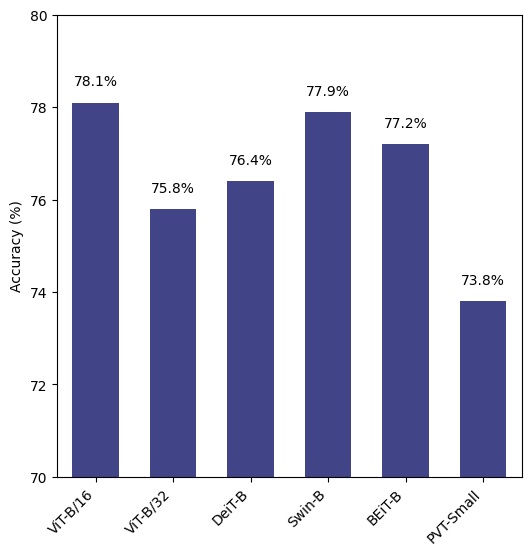
\includegraphics[width=0.6\linewidth]{Figures/pretrained_models.png}
    \caption{Classification Accuracy of Pre-Trained Models}
    \label{fig:pretrained_models}
\end{figure}

Overall, the results confirm that ViT-B/16 remains the most effective model for fine-tuned sleep stage classification, offering the highest accuracy and F1-score. However, models like DeiT-B and Swin-B provide viable alternatives with reasonable accuracy and improved computational efficiency. These findings highlight the trade-offs between model complexity, accuracy, and inference speed, which should be carefully considered in practical applications of automatic sleep stage classification. 

\section{Training and Tuning DCGAN for Synthetic Image Generation}

This section presents the findings on training and tuning DCGAN for synthetic image generation to address subject-to-subject variability and class imbalances in sleep stage classification. The DCGAN architectures listed in Table \ref{tab:dcgan_generator} and Table \ref{tab:discriminator} were trained to generate realistic PSG images, enhancing dataset diversity and improving model generalization. A visual comparison of original and synthetic images is shown in Figure \ref{fig:gan_generated}. The quality of the generated images was evaluated using Structural Similarity Index (SSIM), Fréchet Inception Distance (FID), and Mean Pairwise Euclidean Distance (MPED). The results provide insights into the effectiveness of DCGAN-based augmentation in generating synthetic sleep stage data.

\begin{figure}[H]
    \centering
    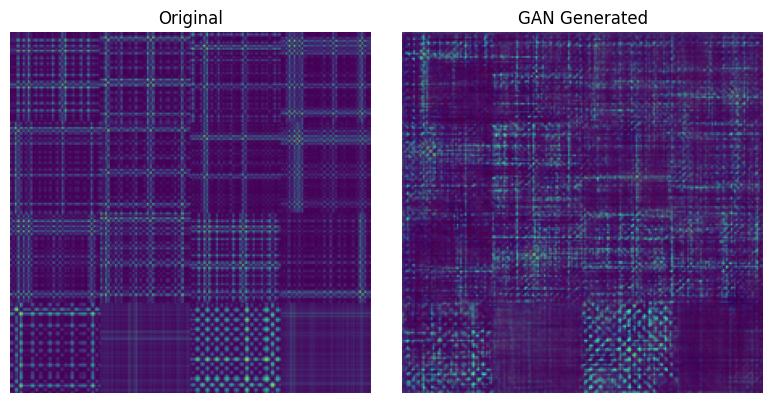
\includegraphics[width=0.6\linewidth]{Figures/gangenerated.png}
    \caption{Original Image vs. GAN Generated Synthetic Image }
    \label{fig:gan_generated}
\end{figure}

According to Figure \ref{fig:gan_generated}, the synthetic sleep stage images retained key structural patterns observed in real GASF transformed images, suggesting that the DCGAN successfully learned essential representations of different sleep stages. However, some variations were noted, such as minor artifacts and slight blurring in certain synthetic samples, which could impact their usefulness in model training. \\

\begin{table}[H]
    \centering
    \resizebox{\textwidth}{!}{ % Ensures the table fits within the page width
    \begin{tabular}{l l c c c c c}
        \toprule
        \textbf{Layer} & \textbf{Type} & \textbf{Kernel Size} & \textbf{Stride} & \textbf{Activation} & \textbf{Normalization} & \textbf{Output Shape} \\
        \midrule
        Input & Random Noise (100-dim) & - & - & - & - & (100,) \\
        Dense & Fully Connected \newline + Reshape & - & - & ReLU & BatchNorm & (14, 14, 1024) \\
        ConvTranspose1 & Transposed Conv2D & 4×4 & 2 & ReLU & BatchNorm & (28, 28, 512) \\
        ConvTranspose2 & Transposed Conv2D & 4×4 & 2 & ReLU & BatchNorm & (56, 56, 256) \\
        ConvTranspose3 & Transposed Conv2D & 4×4 & 2 & ReLU & BatchNorm & (112, 112, 128) \\
        ConvTranspose4 & Transposed Conv2D & 4×4 & 2 & ReLU & BatchNorm & (224, 224, 64) \\
        Output & Transposed Conv2D & 3×3 & 1 & Tanh & - & (224, 224, 3) \\
        \bottomrule
    \end{tabular}
    }
    \caption{DCGAN Generator Architecture}
    \label{tab:dcgan_generator}
\end{table}

\begin{table}[H]
    \centering
    \resizebox{\textwidth}{!}{ % Ensures the table fits within the page width
    \begin{tabular}{l l c c c c c}
        \toprule
        \textbf{Layer} & \textbf{Type} & \textbf{Kernel Size} & \textbf{Stride} & \textbf{Activation} & \textbf{Normalization} & \textbf{Output Shape} \\
        \midrule
        Input & PSG Image (224×224×3) & - & - & - & - & (224, 224, 3) \\
        Conv1 & Conv2D & 4×4 & 2 & LeakyReLU (0.2) & - & (112, 112, 64) \\
        Conv2 & Conv2D & 4×4 & 2 & LeakyReLU (0.2) & BatchNorm & (56, 56, 128) \\
        Conv3 & Conv2D & 4×4 & 2 & LeakyReLU (0.2) & BatchNorm & (28, 28, 256) \\
        Conv4 & Conv2D & 4×4 & 2 & LeakyReLU (0.2) & BatchNorm & (14, 14, 512) \\
        Conv5 & Conv2D & 4×4 & 2 & LeakyReLU (0.2) & BatchNorm & (7, 7, 1024) \\
        Flatten & Fully Connected & - & - & - & - & (1,) \\
        Output & Dense (Sigmoid) & - & - & Sigmoid & - & (1,) \\
        \bottomrule
    \end{tabular}
    }
    \caption{DCGAN Discriminator Architecture}
    \label{tab:discriminator}
\end{table}

We observe an SSIM score of 0.83, indicating high structural fidelity between real and synthetic images. The FID score of 18.7 suggests reasonable realism, though with room for improvement. Additionally, the MPED value of 5.62 confirms sufficient diversity, ensuring that synthetic samples enhance model generalization without redundancy.

\section{Effectiveness of GAN-Augmented Data}

This section presents the findings on the effectiveness of GAN-augmented data for sleep stage classification. The best-performing model, ViT-B/16, was fine-tuned on both the original dataset and a GAN-augmented dataset containing DCGAN-generated synthetic images. Performance comparisons assess whether synthetic data improves classification accuracy and generalization. Figure \ref{fig:synthetic_performance} summarizes the results, providing insights into the impact of GAN-based augmentation.

\begin{figure}[H]
    \centering
    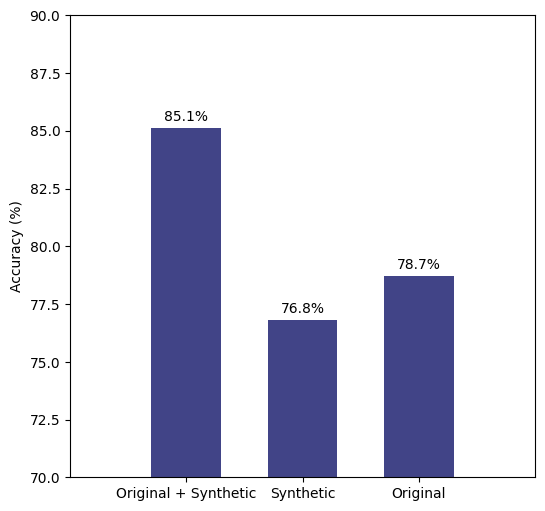
\includegraphics[width=0.6\linewidth]{Figures/synthetic_performance.png}
    \caption{Impact of GAN-Augmented Data on Sleep Stage Classification Performance}
    \label{fig:synthetic_performance}
\end{figure}

The results demonstrate that the combination of original and synthetic data significantly improves classification accuracy, with the mixed dataset yielding an accuracy of 85.1\%. This suggests that GAN-based data augmentation effectively enhances the model’s performance and generalization ability. Although the synthetic dataset alone achieved slightly lower accuracy (76.8\%) than the original dataset (78.7\%), its inclusion in the mixed dataset led to a notable improvement, highlighting the potential of synthetic data in addressing class imbalances and enhancing model robustness.

\section{Final Model}

Following Experiment 6, the ViT-B/16 model trained on the original + synthetic dataset using GASF and DWT at 128 Hz was identified as the best-performing model. To further evaluate its effectiveness, the model was tested on individual sleep stages. Figure \ref{fig:ds9} presents its performance across different sleep stages.

\begin{figure}[H]
    \centering
    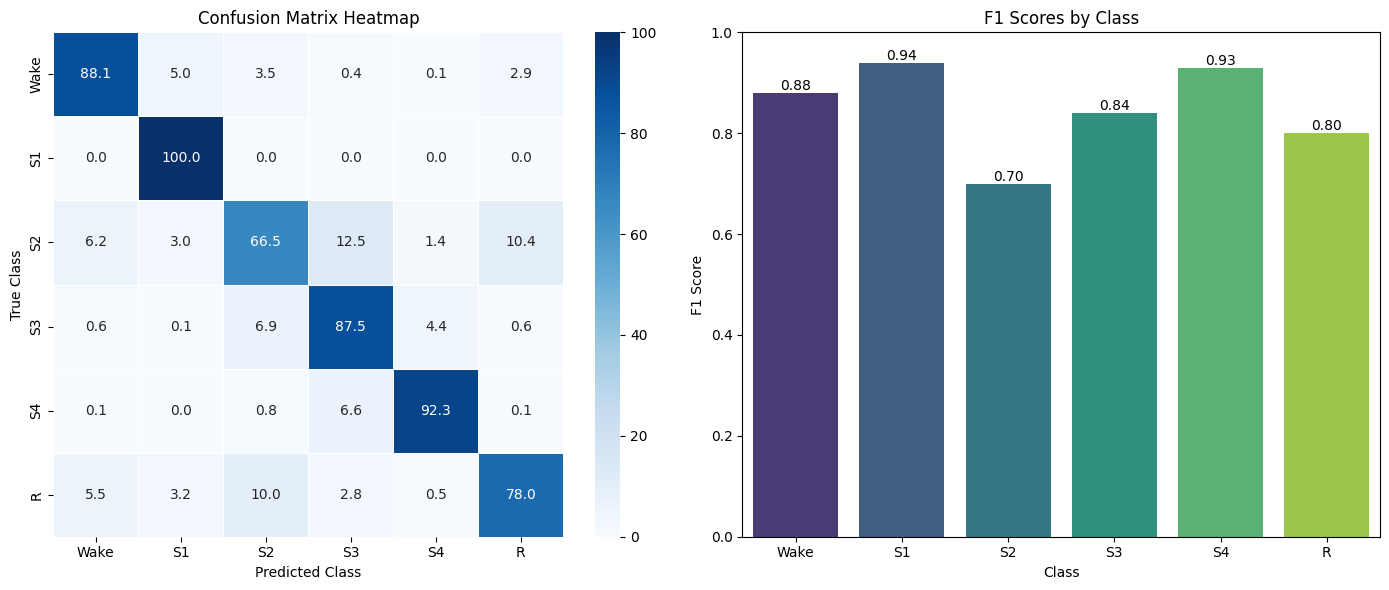
\includegraphics[width=1\linewidth]{Figures/ds9.png}
    \caption{Performance of the Final Model on Individual Sleep Stages}
    \label{fig:ds9}
\end{figure}

The final sleep stage classification model achieved an overall accuracy of 84.8\%, demonstrating its effectiveness in distinguishing between different sleep stages. The confusion matrix and F1 scores provide further insights into the model’s strengths and weaknesses across various classes. \\

The model performed exceptionally well in identifying S1 (light sleep), achieving an F1 score of 0.94, indicating a high balance between precision and recall. Similarly, S4 (deep sleep) was classified with a strong F1 score of 0.92, showing that the model effectively differentiates this stage from others. \\

Wake and REM (Rapid Eye Movement) sleep stages were also predicted with high reliability, obtaining F1 scores of 0.87 and 0.81, respectively. These results indicate the model’s robustness in distinguishing between wakefulness and different sleep states, which is crucial for sleep monitoring applications. \\

However, S3 (a transitional deep sleep stage) exhibited the lowest F1 score of 0.71, suggesting some confusion between S3 and adjacent sleep stages, particularly S2 and S4. The misclassification patterns indicate that the model sometimes confuses lighter and deeper sleep stages, which is a common challenge in sleep stage classification due to the gradual transition between these states. \\

To further assess the generalizability of the proposed sleep stage classification model, we evaluated its performance on the DS1-DS8 datasets. The results, summarized in Table \ref{tab:accuracy}, demonstrate the model's ability to maintain high classification accuracy across diverse datasets.

\begin{table}[H]
    \centering
    \begin{tabular}{|l|c|}
        \hline
        \textbf{DataSet} & \textbf{Accuracy} \\
        \hline
        Healthy (DS1) & 87.9\% \\
        Insomnia (DS2) & 92.8\% \\
        Bruxism (DS3) & 82.4\% \\
        Narcolepsy (DS4) & 88.2\% \\
        NFLE (DS5) & 86.6\% \\
        PLM (DS6) & 85.8\% \\
        RBD (DS7) & 81.0\% \\
        SDB (DS8) & 86.9\% \\
        All Subjects Combined (DS9) & 85.1\% \\
        \hline
    \end{tabular}
    \caption{Accuracy for Different Data Sets}
    \label{tab:accuracy}
\end{table}

The highest accuracy (92.8\%) was achieved on the Insomnia (DS2) dataset, suggesting that the model effectively distinguishes sleep stages in individuals with insomnia, potentially due to the clearer sleep stage transitions in this condition. The model also performed well on Narcolepsy (DS4) and Healthy (DS1) datasets, achieving 88.2\% and 87.9\% accuracy, respectively, demonstrating its effectiveness in both normal and disordered sleep patterns. \\

However, slightly lower accuracies were observed in datasets representing Bruxism (DS3, 82.4\%) and REM Behavior Disorder (RBD, DS7, 81.0\%), suggesting potential challenges in distinguishing sleep stages in subjects with these conditions. These variations could be attributed to irregular sleep patterns, movement artifacts, or differences in EEG characteristics associated with these disorders.\\

Despite these challenges, the model maintains strong generalization across all datasets, with accuracy ranging from 81.0\% to 92.8\%, reinforcing its applicability for diverse sleep conditions. 

\chapter{Conclusion}

\section{Conclusion}

This study aimed to explore the effectiveness of Vision Transformers (ViTs) for sleep stage classification, particularly focusing on improving model performance through various image transformation techniques, sampling frequencies, pre-trained models, and data augmentation methods. Through a series of experiments, we identified the optimal model and approach for classifying sleep stages using PSG signals. The ViT-B/16 model fine-tuned on the combined original and synthetic dataset with GASF and DWT at 128 Hz emerged as the best performer, demonstrating its ability to classify sleep stages with high accuracy and generalization capability. \\

Our findings align with previous studies highlighting the effectiveness of deep learning models, particularly ViTs, in handling complex time-series data like PSG signals. The use of synthetic data generated by DCGAN also proved beneficial, suggesting that GAN-based augmentation can help mitigate issues related to class imbalances and subject-to-subject variability. These results contribute to the growing body of research that emphasizes the potential of deep learning models, particularly ViTs, in enhancing the accuracy of sleep stage classification. \\

Despite the promising results, a few unexpected findings were observed, such as slight degradation in accuracy when using only synthetic data. While the GAN-augmented dataset led to a substantial improvement when combined with the original data, the performance of synthetic-only data was lower than expected. This highlights the need for further optimization in the GAN generation process to ensure more reliable synthetic data.

\section{Limitations}

While this study demonstrates the potential of Vision Transformers for sleep stage classification, several limitations should be acknowledged. One key limitation is the limited dataset scope—although the model was evaluated on DS1–DS8 datasets, its performance may not generalize to all sleep conditions or populations. Larger and more diverse datasets are needed to validate its robustness further. Another limitation is the quality of synthetic data generated by the GAN model. While synthetic data helped mitigate class imbalance, it was not entirely reliable when used independently, suggesting a need for more advanced GAN architectures to improve data fidelity. Additionally, the computational complexity of Vision Transformers presents a challenge for real-time deployment, particularly in wearable sleep monitoring devices, where efficiency and low power consumption are critical. \\

Furthermore, despite achieving high accuracy, the model's lack of interpretability remains a concern. Since deep learning models, including ViTs, function as black boxes, understanding their decision-making process is difficult. Future studies should incorporate explainability techniques such as attention visualization or SHAP analysis to enhance trust in clinical applications. Another limitation is the focus on EEG signals, as PSG data also includes other physiological signals like ECG, EOG, and EMG, which were not fully explored in this study. The integration of these additional modalities could potentially improve classification performance. Lastly, the study relied on fixed hyperparameters, without extensive optimization across different datasets. A more systematic hyperparameter tuning approach could further refine the model’s performance, ensuring better adaptation to varying sleep conditions. Addressing these limitations in future work could enhance the model’s reliability, interpretability, and practical applicability in real-world sleep monitoring scenarios.

\section{Further Work}

While the findings of this study provide valuable insights into the use of Vision Transformers for sleep stage classification, there are several areas where further research can build upon this work.

\begin{enumerate}
    \item \textbf{Improving GAN Generation Quality}: Future work could focus on improving the quality of synthetic data generated by DCGAN, potentially exploring advanced GAN architectures like StyleGAN or conditional GANs (cGANs) to reduce artifacts and blurring in the generated images.
    \item \textbf{Larger and More Diverse Datasets}: To further test the generalization capability of the model, future research could involve training and evaluating the model on a larger and more diverse set of datasets, beyond DS1–DS8, to assess its robustness across varied populations and sleep conditions.
    \item \textbf{Real-World Data Applications}: The practical implications of the model’s performance in real-world sleep studies should be explored. Evaluating the model on datasets from different clinical settings or using long-term sleep data from wearable devices would provide insights into the applicability of this approach in real-world environments.
    \item \textbf{Hybrid Models}: Investigating hybrid models combining ViTs with other deep learning techniques, such as Convolutional Neural Networks (CNNs) or Recurrent Neural Networks (RNNs), could potentially enhance performance, especially for sequential data.
    \item \textbf{Exploring Interpretability}: Although this study did not focus on interpretability, future research could look into explaining model predictions, which is particularly important in medical domains where understanding model decisions can be critical for clinical applications.
\end{enumerate}
By addressing these areas, future research can further advance the field of sleep stage classification, making it more accurate, reliable, and applicable for real-world use. \cite{mohomed2024nocturne}

 

\chapter*{Appendices}

\section*{Appendix A : GitHub Repository for Code}

The code used for preprocessing, model training, evaluation, and analysis in this thesis is available at the following GitHub repository:

\textbf{GitHub Link:} 
\url{https://github.com/JanithRavinduRashmika/EEG_Sleep_Stage}

The repository contains:

\begin{itemize}
    \item Python scripts for PSG data preprocessing and transformation.
    \item Code for implementing and fine-tuning Vision Transformer models.
    \item Jupyter notebooks demonstrating model training and evaluation.
\end{itemize}

\section*{Appendix B : PSG Data Access}

The CAP Sleep Database, used for the sleep stage classification experiments in this thesis, is available on PhysioNet at the following link: 
\url{https://physionet.org/content/capslpdb/1.0.0/}


This database contains polysomnographic (PSG) recordings from multiple subjects, which include EEG, ECG, and EOG signals for sleep stage classification tasks. Researchers can access this data by registering for an account on PhysioNet.
 
\addtocontents{toc}{\vspace{1em}}
\addcontentsline{toc}{section}{Appendices}

\printbibliography
\addtocontents{toc}{\vspace{1em}}
\addcontentsline{toc}{section}{Bibliography}

\end{document}
